% Options for packages loaded elsewhere
\PassOptionsToPackage{unicode}{hyperref}
\PassOptionsToPackage{hyphens}{url}
\documentclass[
  english,
  10pt]{article}
\usepackage{xcolor}
\usepackage{amsmath,amssymb}
\setcounter{secnumdepth}{-\maxdimen} % remove section numbering
\usepackage{iftex}
\ifPDFTeX
  \usepackage[T1]{fontenc}
  \usepackage[utf8]{inputenc}
  \usepackage{textcomp} % provide euro and other symbols
\else % if luatex or xetex
  \usepackage{unicode-math} % this also loads fontspec
  \defaultfontfeatures{Scale=MatchLowercase}
  \defaultfontfeatures[\rmfamily]{Ligatures=TeX,Scale=1}
\fi
\usepackage{lmodern}
\ifPDFTeX\else
  % xetex/luatex font selection
\fi
% Use upquote if available, for straight quotes in verbatim environments
\IfFileExists{upquote.sty}{\usepackage{upquote}}{}
\IfFileExists{microtype.sty}{% use microtype if available
  \usepackage[]{microtype}
  \UseMicrotypeSet[protrusion]{basicmath} % disable protrusion for tt fonts
}{}
\makeatletter
\@ifundefined{KOMAClassName}{% if non-KOMA class
  \IfFileExists{parskip.sty}{%
    \usepackage{parskip}
  }{% else
    \setlength{\parindent}{0pt}
    \setlength{\parskip}{6pt plus 2pt minus 1pt}}
}{% if KOMA class
  \KOMAoptions{parskip=half}}
\makeatother
\usepackage{color}
\usepackage{fancyvrb}
\newcommand{\VerbBar}{|}
\newcommand{\VERB}{\Verb[commandchars=\\\{\}]}
\DefineVerbatimEnvironment{Highlighting}{Verbatim}{commandchars=\\\{\}}
% Add ',fontsize=\small' for more characters per line
\newenvironment{Shaded}{}{}
\newcommand{\AlertTok}[1]{\textcolor[rgb]{1.00,0.00,0.00}{\textbf{#1}}}
\newcommand{\AnnotationTok}[1]{\textcolor[rgb]{0.38,0.63,0.69}{\textbf{\textit{#1}}}}
\newcommand{\AttributeTok}[1]{\textcolor[rgb]{0.49,0.56,0.16}{#1}}
\newcommand{\BaseNTok}[1]{\textcolor[rgb]{0.25,0.63,0.44}{#1}}
\newcommand{\BuiltInTok}[1]{\textcolor[rgb]{0.00,0.50,0.00}{#1}}
\newcommand{\CharTok}[1]{\textcolor[rgb]{0.25,0.44,0.63}{#1}}
\newcommand{\CommentTok}[1]{\textcolor[rgb]{0.38,0.63,0.69}{\textit{#1}}}
\newcommand{\CommentVarTok}[1]{\textcolor[rgb]{0.38,0.63,0.69}{\textbf{\textit{#1}}}}
\newcommand{\ConstantTok}[1]{\textcolor[rgb]{0.53,0.00,0.00}{#1}}
\newcommand{\ControlFlowTok}[1]{\textcolor[rgb]{0.00,0.44,0.13}{\textbf{#1}}}
\newcommand{\DataTypeTok}[1]{\textcolor[rgb]{0.56,0.13,0.00}{#1}}
\newcommand{\DecValTok}[1]{\textcolor[rgb]{0.25,0.63,0.44}{#1}}
\newcommand{\DocumentationTok}[1]{\textcolor[rgb]{0.73,0.13,0.13}{\textit{#1}}}
\newcommand{\ErrorTok}[1]{\textcolor[rgb]{1.00,0.00,0.00}{\textbf{#1}}}
\newcommand{\ExtensionTok}[1]{#1}
\newcommand{\FloatTok}[1]{\textcolor[rgb]{0.25,0.63,0.44}{#1}}
\newcommand{\FunctionTok}[1]{\textcolor[rgb]{0.02,0.16,0.49}{#1}}
\newcommand{\ImportTok}[1]{\textcolor[rgb]{0.00,0.50,0.00}{\textbf{#1}}}
\newcommand{\InformationTok}[1]{\textcolor[rgb]{0.38,0.63,0.69}{\textbf{\textit{#1}}}}
\newcommand{\KeywordTok}[1]{\textcolor[rgb]{0.00,0.44,0.13}{\textbf{#1}}}
\newcommand{\NormalTok}[1]{#1}
\newcommand{\OperatorTok}[1]{\textcolor[rgb]{0.40,0.40,0.40}{#1}}
\newcommand{\OtherTok}[1]{\textcolor[rgb]{0.00,0.44,0.13}{#1}}
\newcommand{\PreprocessorTok}[1]{\textcolor[rgb]{0.74,0.48,0.00}{#1}}
\newcommand{\RegionMarkerTok}[1]{#1}
\newcommand{\SpecialCharTok}[1]{\textcolor[rgb]{0.25,0.44,0.63}{#1}}
\newcommand{\SpecialStringTok}[1]{\textcolor[rgb]{0.73,0.40,0.53}{#1}}
\newcommand{\StringTok}[1]{\textcolor[rgb]{0.25,0.44,0.63}{#1}}
\newcommand{\VariableTok}[1]{\textcolor[rgb]{0.10,0.09,0.49}{#1}}
\newcommand{\VerbatimStringTok}[1]{\textcolor[rgb]{0.25,0.44,0.63}{#1}}
\newcommand{\WarningTok}[1]{\textcolor[rgb]{0.38,0.63,0.69}{\textbf{\textit{#1}}}}
\usepackage{longtable,booktabs,array}
\usepackage{caption}
\captionsetup[table]{skip=6pt}
\newcounter{none} % for unnumbered tables
\usepackage{calc} % for calculating minipage widths
% Correct order of tables after \paragraph or \subparagraph
\usepackage{etoolbox}
\makeatletter
\patchcmd\longtable{\par}{\if@noskipsec\mbox{}\fi\par}{}{}
\makeatother
\usepackage{graphicx}
\makeatletter
\newsavebox\pandoc@box
\newcommand*\pandocbounded[1]{% scales image to fit in text height/width
  \sbox\pandoc@box{#1}%
  \Gscale@div\@tempa{\textheight}{\dimexpr\ht\pandoc@box+\dp\pandoc@box\relax}%
  \Gscale@div\@tempb{\linewidth}{\wd\pandoc@box}%
  \ifdim\@tempb\p@<\@tempa\p@\let\@tempa\@tempb\fi% select the smaller of both
  \ifdim\@tempa\p@<\p@\scalebox{\@tempa}{\usebox\pandoc@box}%
  \else\usebox{\pandoc@box}%
  \fi%
}
% Set default figure placement to htbp
\def\fps@figure{htbp}
\makeatother
\ifLuaTeX
\usepackage[bidi=basic,shorthands=off]{babel}
\else
\usepackage[bidi=default,shorthands=off]{babel}
\fi
\ifLuaTeX
  \usepackage{selnolig} % disable illegal ligatures
\fi
\setlength{\emergencystretch}{3em} % prevent overfull lines
\providecommand{\tightlist}{%
  \setlength{\itemsep}{0pt}\setlength{\parskip}{0pt}}
% Preamble extras — DFRWS / FSI:DI–inspired article look (pandoc -H)
\usepackage{microtype}
\usepackage{booktabs}
\usepackage{longtable}
\usepackage{tabularx}
\usepackage{array}
\usepackage{multirow}
\usepackage{float}
\usepackage{xcolor}
\usepackage{xurl}
\usepackage{seqsplit}
\usepackage{fancyhdr}
\usepackage{titlesec}
\usepackage{hyperref}
\Urlmuskip=0mu plus 1mu
\newcolumntype{Y}{>{\raggedright\arraybackslash}X}
\definecolor{JournalBlue}{HTML}{003366}
\hypersetup{
  colorlinks=true,
  linkcolor=black!70!blue,
  citecolor=black!70!blue,
  urlcolor=black!60!teal,
  pdftitle={From GrandSlam to MMCS: Modern Apple Private Protocols for Authentication, Escrow/PCS, Octagon/CKKS, and iCloud Device Backup Acquisition},
  pdfauthor={Giordano Sconti},
  pdfsubject={Technical whitepaper — GrandSlam, Escrow, Octagon, CKKS, MMCS},
  pdfkeywords={GrandSlam, EscrowProxy, Octagon, CKKS, Manatee, MMCS, PCSMMCS2, ADP, Mobile forensics}
}
\usepackage{geometry}
\geometry{a4paper,left=2.0cm,right=2.0cm,top=2.4cm,bottom=2.2cm}
\setlength{\parskip}{0.4em}
\setlength{\parindent}{0pt}
\renewcommand{\arraystretch}{1.12}
\floatplacement{figure}{H}

% Running header / footer (skip first page via fancy)
\pagestyle{fancy}
\fancyhf{}
\fancyhead[L]{\footnotesize\color{gray} G. Sconti / From GrandSlam to MMCS}
\fancyhead[R]{\footnotesize\color{gray} Whitepaper 1.11}
\fancyfoot[L]{\footnotesize\color{gray} Digital forensics · Apple iCloud protocols}
\fancyfoot[R]{\footnotesize\color{gray}\thepage}
\renewcommand{\headrulewidth}{0.4pt}
\renewcommand{\footrulewidth}{0.4pt}
\fancypagestyle{plain}{%
  \fancyhf{}%
  \fancyfoot[L]{\footnotesize\color{gray} Digital forensics · Apple iCloud protocols}%
  \fancyfoot[R]{\footnotesize\color{gray}\thepage}%
  \renewcommand{\headrulewidth}{0pt}%
  \renewcommand{\footrulewidth}{0.4pt}%
}

\titleformat{\section}{\large\bfseries}{\thesection}{0.8em}{}
\titleformat{\subsection}{\normalsize\bfseries}{\thesubsection}{0.7em}{}
\titleformat{\subsubsection}{\normalsize\itshape\bfseries}{\thesubsubsection}{0.6em}{}
\titlespacing*{\section}{0pt}{1.2em}{0.45em}
\titlespacing*{\subsection}{0pt}{0.9em}{0.3em}
\usepackage{bookmark}
\IfFileExists{xurl.sty}{\usepackage{xurl}}{} % add URL line breaks if available
\urlstyle{same}
% fallback for those not using the hyperref driver hyperxmp:
\makeatletter
\@ifundefined{xmpquote}{\newcommand{\xmpquote}[1]{#1}}{}
\makeatother
\hypersetup{
  pdflang={en},
  hidelinks,
  pdfcreator={LaTeX via pandoc}}

\author{}
\date{}

\begin{document}

\section{From GrandSlam to MMCS: A Description of Modern Apple Private
Protocols for Authentication, Escrow/PCS, Octagon/CKKS, and iCloud
Device Backup
Acquisition}\label{from-grandslam-to-mmcs-a-description-of-modern-apple-private-protocols-for-authentication-escrowpcs-octagonckks-and-icloud-device-backup-acquisition}

Giordano Sconti\\
Gruppo Informatici Forensi\\
\emph{Corresponding author:} giordano.sconti@gruppoinformaticiforensi.it

16 November 2026 · Version 1.11 · Based on authorized experimental
observation (owned accounts / forensic mandate)

\subsection{Abstract}\label{abstract}

Commercial iCloud acquisition tools often prove insufficient when
\textbf{iCloud.com is disabled}, \textbf{Advanced Data Protection (ADP)}
is enabled, or \textbf{Lockdown Mode} restricts available client
surfaces. Under such conditions, acquisition cannot rely on web APIs but
requires combining Apple private protocols: authentication via
\textbf{GrandSlam / GsService2}, cryptographic material retrieval
through \textbf{EscrowProxy} and/or \textbf{Octagon / Cuttlefish},
opening of \textbf{CKKS} (\emph{CloudKit Keychain Syncing}) views, with
particular attention to \textbf{Manatee} and \textbf{TLKShare},
inventory of backups within the CloudKit zone \textbf{\texttt{mbksync}},
and finally transfer of \textbf{MMCS} chunks using the \textbf{PCSMMCS2}
derivation.

This whitepaper provides an organized description of such protocols, as
reconstructed and verified in the open-source project \emph{iCloudKit
Extractor} (IKE) from March to November 2026. The contribution is
analytical: (i) distinguish the \textbf{recovery paths} Escrow PCS
(\texttt{dsid:dsid}), Escrow iCDP, and Recovery Key; (ii) clarify the
role of \textbf{Manatee / TLKShare} as the source of PCS material for
backups protected by ADP; (iii) document the sequence \textbf{Lock →
authorizeGet → FileGroups → Ford / ChunkInfo}; (iv) situate the recovery
path within a forensic model that is accountable.

\textbf{Appendix A} describes the reverse engineering methodology
adopted (thesis on obfuscation/DBI as a map, x64dbg/MCP on virtualized
regions, Frida on \texttt{memcpy} for capturing payloads such as
\texttt{dsid:dsid}), without providing procedures for bypassing software
protections nor for accessing unauthorized accounts.

\textbf{Keywords:} Mobile forensics; Cloud forensics; Cloud acquisition;
GrandSlam; GsService2; EscrowProxy; PCS; iCDP; Octagon; Cuttlefish;
CKKS; Manatee; TLKShare; MMCS; PCSMMCS2; ADP; iCloud backup.

\begin{center}\rule{0.5\linewidth}{0.5pt}\end{center}

\subsection{1. Introduction}\label{introduction}

\subsubsection{1.1 Problem}\label{problem}

The acquisition of an \textbf{iCloud device backup} is not a monolithic
operation. From a commercial perspective, it is often presented as
authentication followed by download; from a protocol standpoint, it is a
\textbf{staged pipeline}, each stage featuring its own authentication,
state, and failure modes. When the account has \textbf{ADP} enabled,
backup data and most of the CloudKit content remain client-side
encrypted until adequate \textbf{PCS} material is obtained---typically
through the \textbf{Octagon} trust domain (an iCDP record with the
device passcode, or a \textbf{Recovery Key}).

In March 2026, within an experimental laboratory setting, the need to
recover a backup with ADP was not met by the forensic commercial tools
available at the time. This motivated a seven-month research effort,
culminating in stable acquisitions (ADP enabled or disabled) and the
experimental publication of IKE.

\subsubsection{1.2 Objectives of the
document}\label{objectives-of-the-document}

\begin{enumerate}
\def\labelenumi{\arabic{enumi}.}
\tightlist
\item
  \textbf{Describe} the Backup / Octagon / PCS protocols starting from
  GrandSlam.
\item
  \textbf{Distinguish} often confused concepts in non-peer-reviewed
  sources (\texttt{dsid:dsid} vs passcode iCDP vs Recovery Key).
\item
  \textbf{Establish} the protocol invariants still valid as of November
  2026, while recognizing that Apple may modify private surfaces.
\item
  \textbf{Document}, in the appendix, the reconstruction methodology in
  a form suitable for academic evaluation.
\end{enumerate}

\subsubsection{1.3 What this whitepaper is
not}\label{what-this-whitepaper-is-not}

It is not an IKE usage manual, nor an exhaustive commercial comparison,
nor a guide to unauthorized access. It does not cover generic CloudKit
or any other surfaces unnecessary to the device backup acquisition
chain.

\subsubsection{1.4 Structure}\label{structure}

Sections 2--3 frame the problem and present the chain. Sections 4--11
delve into each stage (including Domain/\texttt{fileList} inventory in
Section 9.5). Section 12 consolidates pathways and limitations. Section
13 provides UML sequence diagrams and request/response skeletons (Figure
11 for file lists). Appendix A outlines the methodology.

\begin{center}\rule{0.5\linewidth}{0.5pt}\end{center}

\subsection{2. Context, operational model and related
works}\label{context-operational-model-and-related-works}

\subsubsection{2.1 Operational model}\label{operational-model}

An \textbf{authorized operator} (Apple ID holder or party duly
authorized by forensic mandate) shall:

\begin{itemize}
\tightlist
\item
  possesses Apple ID credentials and, if required, the \textbf{device
  passcode} used when the iCDP record was created and/or the
  \textbf{Recovery Key};
\item
  can complete the GrandSlam authentication with coherent Anisette
  identity;
\item
  does not perform brute-force attacks against the HSM record Escrow
  limits;
\item
  uses the output (an iTunes-compatible tree) for legitimate forensic
  analysis.
\end{itemize}

Compared to Apple's threat model for which such mechanisms are designed,
a remote attacker possessing only session tokens, without Octagon/PCS
material, should not be able to decrypt data protected by ADP: ADP
raises the barrier by specifically requiring material that does not
reside solely in the \texttt{mmeAuthToken}.

\subsubsection{2.2 Why web paths are not
sufficient}\label{why-web-paths-are-not-sufficient}

Authentication via \textbf{iCloud.com / idmsa} generates tokens useful
for browser surfaces (e.g., Photos web, some SMS/trusted-device flows).
Such tokens \textbf{do not} equate to the mobile / AuthKit session
required by EscrowProxy, Cuttlefish, and Mobile Backup. Confusing the
two planes is a common error: a seemingly valid access is obtained,
followed by 403 responses or empty inventories on \texttt{mbksync} or
Escrow.

\subsubsection{2.3 Related Work}\label{related-work}

Academic literature and public disclosures address
iCloud/backup/CloudKit from distinct perspectives. To our knowledge,
none provides an open-ended end-to-end description of the contemporary
chain \emph{GrandSlam → Escrow/Octagon → \texttt{mbksync} Lock →
MMCS/\texttt{PCSMMCS2}}. The following are relevant lines of inquiry;
complete references are in Section 16.

\paragraph{2.3.1 Forensics on local backups and cloud
acquisition}\label{forensics-on-local-backups-and-cloud-acquisition}

Geus, Ottmann, and Freiling systematically evaluate the forensic
suitability of local iOS/Android backups and observe that forensic
access to remote backups on iCloud/Google Drive is ``complicated, or in
some instances impossible'' {[}1{]}. The contribution is methodological
regarding the integrity of local acquisition; it does not reconstruct
Apple's cloud protocols.

Geus, Gruber, Wozar, and Freiling (DFRWS APAC 2025 / \emph{Forensic
Science International: Digital Investigation}) compare local backups,
full file system extractions, and iCloud restore via \emph{dynamic
binary instrumentation}, highlighting discrepancies in timestamps and
minor user data differences {[}21{]}. The study evaluates the accuracy
and completeness of \emph{cloud backup restore} on the intermediate
device; it does not describe the private protocol chain GrandSlam →
Escrow/Octagon → \texttt{mbksync} → MMCS used by a direct acquisition
client.

Roussev, Barreto, and Ahmed introduce forensic acquisition of
\textbf{cloud drives} based on APIs, emphasizing generic remote
acquisition models rather than contemporary Mobile Backup iCloud
{[}2{]}. Zinkus, Jois, and Green provide a state-of-the-art review on
\textbf{mobile device security}, mentioning CloudKit and the key
hierarchy (CloudKit Service Key / synchronized Keychain) at the
architectural level, without a backup download protocol {[}3{]}.

These works \textbf{frame the problem} (restore integrity, cloud backup
scope, generic API acquisition) but leave open the protocol gap
addressed in this document.

\paragraph{2.3.2 Industrial disclosures on iCloud
protocols}\label{industrial-disclosures-on-icloud-protocols}

Katalov (ElcomSoft) presents at HITB 2013 the first public,
comprehensive analysis of the then-in-use iCloud protocols:
authentication, Mobile Backup Service, chunking, and
\texttt{authorizeGet} to third-party storage {[}4{]}. A variant of the
same material appears at REcon 2013 {[}5{]}. The model described
predates the CloudKit catalog centered on \texttt{mbksync} and the
\texttt{D:}--\texttt{S:}--Lock records, and does not include ADP or
Octagon.

At HITB 2018, Katalov documents the extraction of \textbf{Messages in
iCloud} via CloudKit (\texttt{com.apple.messages.cloud}), referencing
the Manatee zones and the PCS/Engram materials, as well as the
\emph{Ford chunks} {[}6{]}. The focus is on Messages/Keychain
synchronization, not on full device backup in the presence of ADP. A
related presentation on iCloud Keychain appears at SecTor 2017 {[}7{]}.

These disclosures constitute the most recent public precedents on a
protocol level; the present work extends them to the device backup
pathway 2024--2026 and to the taxonomy of recovery pathways.

\paragraph{2.3.3 Official documentation and teaching
materials}\label{official-documentation-and-teaching-materials}

The \emph{Apple Platform Security Guide} describes escrow and recovery
of \textbf{iCloud Keychain} (cluster HSM / Cloud Key Vault, attempt
limits, SRP on the \emph{iCloud security code}) {[}8{]}, {[}9{]}. The
IAIK course slides (TU Graz) reuse the same model for pedagogical
purposes, highlighting the lack of details regarding encryption of
\emph{full iCloud backups} {[}10{]}.

Such sources are authoritative on the \textbf{Keychain security model},
not on the \texttt{mbksync} → MMCS protocol flow.

\paragraph{2.3.4 Open-source software and experimental
observation}\label{open-source-software-and-experimental-observation}

IKE is an independent implementation in C\#, developed in isolation from
the code of observed commercial clients. As a cross-check of
nomenclature and flow patterns (without incorporation of third-party
code), the following were consulted: appleservices {[}11{]},
iCloud-Keychain-for-Linux {[}12{]}, rustpush (SSPL license; limited to
study only) {[}13{]}, and fragments of Apple OSS TrustedPeersHelper for
the KDF of the Recovery Key {[}14{]}. The initial orientation toward
Escrow/MMCS utilized experimental observation of \textbf{Elcomsoft Phone
Breaker} under legitimate license {[}15{]}; attribution boundaries are
defined in \texttt{NOTICE.md} {[}16{]}. A capability matrix (snapshot)
is available in {[}17{]}.

\subsubsection{2.4 Contribution with respect to the state of the
art}\label{contribution-with-respect-to-the-state-of-the-art}

In contrast to {[}1{]}, {[}21{]} and {[}2{]}--{[}3{]}, this contribution
is not an integrity/completeness assessment of the restore on an
intermediate device, but rather a \textbf{protocol-level map of the
remote direct acquisition pathway} that these venues declare difficult,
opaque, or out of scope. In contrast to {[}4{]}--{[}7{]}, the analysis
is updated and specialized to the backup device in the presence of ADP
and to distinct recovery pathways. In contrast to {[}8{]}--{[}10{]}, the
approach moves from the Keychain escrow model to the CloudKit/MMCS
protocol.

In summary, IKE and this white paper make inspectable: (i) the
distinction between PCS Escrow / iCDP / Recovery Key; (ii) Manatee as
the source of PCS material for ADP; (iii) the sequence Lock →
authorizeGet → FileGroups → Ford/ChunkInfo, with IKM from
\texttt{protectionInfo} and salt \texttt{PCSMMCS2}---elements missing or
only partially addressed in the open literature cited.

\subsubsection{2.5 Experimental evidence
(synthesis)}\label{experimental-evidence-synthesis}

During 2026, the laboratory verified the following on accounts owned by
the researchers:

\begin{itemize}
\tightlist
\item
  listing and locking on concurrent backups (including scenarios in
  which commercial tools returned \emph{Access Denied} / 403 with
  iCloud.com disabled and ADP enabled);
\item
  download MMCS protocol-complete after correction of the lead
  classifier for \texttt{0xC4} (August);
\item
  ADP opening via iCDP passcode (October) and via Recovery Key →
  TLKShares (October);
\item
  materialization of trees recognized by forensic tools as layout
  compatible with iTunes.
\end{itemize}

Micro-benchmarks of throughput are not provided: the focus of this
whitepaper is protocol correctness, not network performance. The Day
1--11 laboratory notes constitute the underlying experimental log
{[}19{]}.

\subsubsection{2.6 Informal and non-peer-reviewed
sources}\label{informal-and-non-peer-reviewed-sources}

Alongside {[}1{]}--{[}10{]}, there is extensive informal discussion
(forum, gist, legacy tools) on ``downloading iCloud''. Most of that
material:

\begin{itemize}
\tightlist
\item
  is prior to the contemporary CloudKit/\texttt{mbksync} model (and
  often also relative to {[}4{]}, {[}5{]});
\item
  does not distinguish recovery paths of Escrow;
\item
  does not document IKM/\texttt{PCSMMCS2};
\item
  reduces ADP to a generic «device code is required», without
  distinguishing between iCDP, Recovery Key, and PCS Escrow.
\end{itemize}

This work falls within the tradition of protocol reverse engineering
technical reports, where value lies in the reproducibility of the
documented invariants presented in {[}18{]}, {[}19{]}.

\subsubsection{2.7 Terminological alignment notes with respect to the
sources}\label{terminological-alignment-notes-with-respect-to-the-sources}

Following the comparison with {[}4{]}--{[}10{]} and with the open-source
Apple/community documentation {[}11{]}--{[}14{]}, the following
inconsistencies are identified and corrected with respect to previous
internal drafts:

\begin{itemize}
\tightlist
\item
  \emph{OpenVault} as a protocol name in Apple → \textbf{does not
  appear} in {[}8{]}--{[}10{]} (laboratory label). It is used for
  \emph{opening CKKS views}.
\item
  \emph{seed PCS} → laboratory metaphor. It uses \emph{session PCS
  material}.
\item
  \emph{Escrow} path applied also to the Recovery Key → the RK
  \textbf{does not} use EscrowProxy \texttt{RECOVER} {[}12{]}, {[}14{]}.
  The \emph{recovery path} is used (Escrow only for A/B).
\item
  \emph{spine} / \emph{ladder} / \emph{gate} / \emph{pipe} → reverse
  engineering jargon. The terms \emph{chain}, \emph{sequence}, and
  \emph{transport} are used.
\item
  \emph{oracle} / \emph{reimplementation} → laboratory log language.
  \emph{Observational reference} and \emph{independent implementation}
  are used.
\item
  Manatee ≡ Engram → distinct views; Engram typically messages {[}6{]}.
  Manatee = PCS source for ADP; Engram outside backup path.
\item
  \emph{CKKS} without expansion → ambiguity. Expands to \emph{CloudKit
  Keychain Syncing}.
\end{itemize}

The term \textbf{Ford}, used in Section 10, is retained because it
appears already in public disclosures on Messages/CloudKit {[}6{]}; it
is not a neologism introduced in this work.

\begin{center}\rule{0.5\linewidth}{0.5pt}\end{center}

\subsection{3. Protocol Chain Overview}\label{protocol-chain-overview}

The acquisition session is a \textbf{staged pipeline} (Figure 1). Each
transition admits its own failures: a valid GrandSlam token does not
imply an open keybag; a recovered iCDP record does not imply a complete
\texttt{authorizeGet}; a complete \texttt{authorizeGet} does not imply
correct Ford decryption if the IKM is incorrect.

\pandocbounded{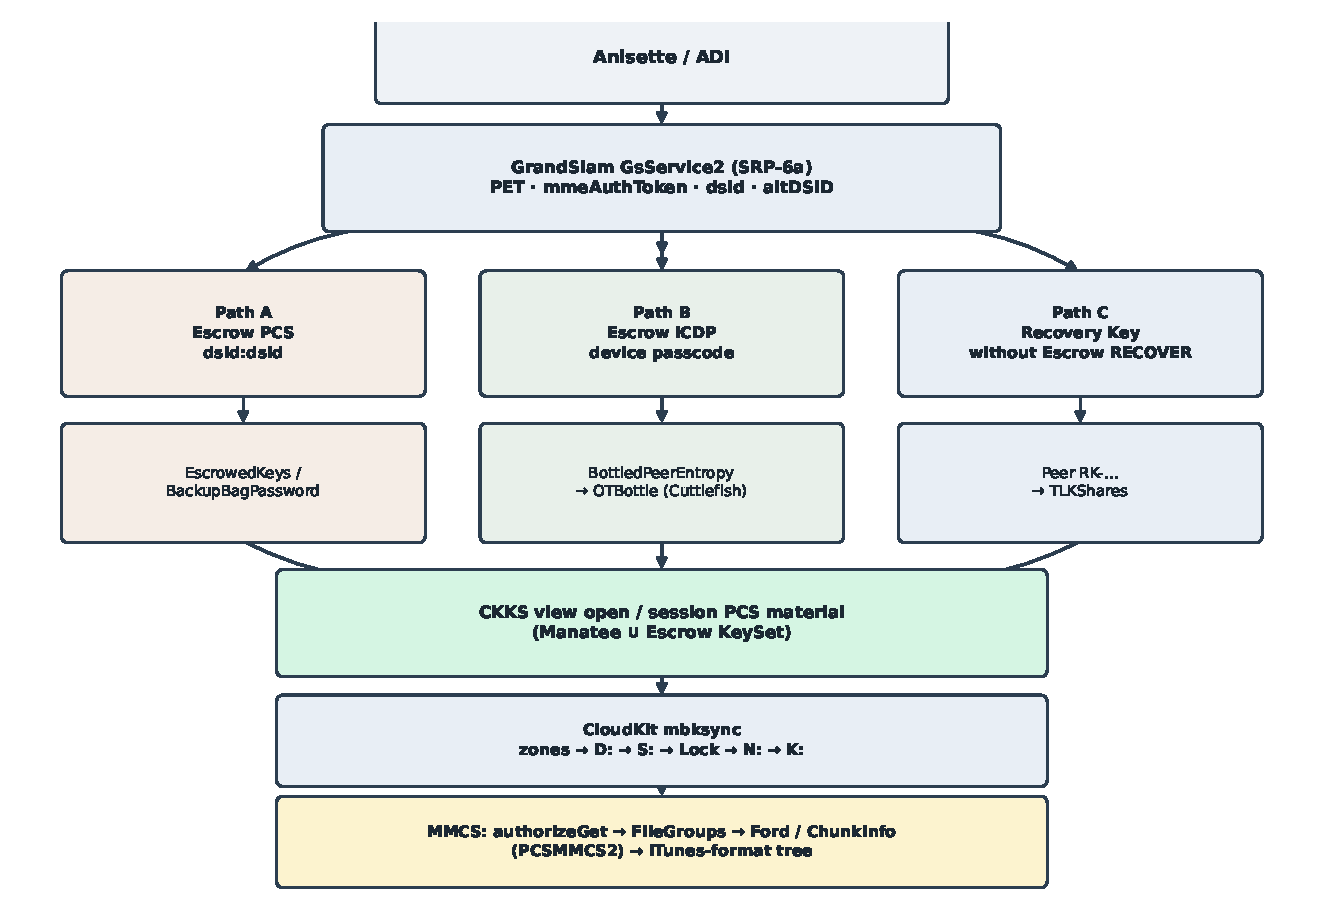
\includegraphics[keepaspectratio]{figures/fig01-catena-end-to-end.pdf}}

\textbf{Figure 1.} End-to-end panorama: Anisette → GrandSlam → three
recovery paths → PCS material → \texttt{mbksync} → MMCS →
iTunes-formatted tree.

\begin{center}\rule{0.5\linewidth}{0.5pt}\end{center}

\subsection{4. Precondition: Anisette /
ADI}\label{precondition-anisette-adi}

Before GsService2, the client presents \textbf{Anisette} headers of the
family \texttt{X-Apple-I-MD*}, derived from an ADI (\texttt{akd} /
provisioning) stack consistent with the declared device profile.
Anisette alone does not open a backup: it is the \textbf{protocol
identity} without which Apple rejects or degrades non-browser clients.

\subsubsection{4.1 MidService machine
provisioning}\label{midservice-machine-provisioning}

On real iPhone/\texttt{akd} traffic, Anisette material is minted through
GrandSlam \textbf{MidService} \emph{before} usable \texttt{X-Apple-I-MD}
/ \texttt{X-Apple-I-MD-M} headers exist {[}22{]}. The reconstructed
order is:

\begin{verbatim}
lookup (url bag)
  → startMachineProvisioning  → spim
  → [local] ADIProvisioningStart(spim, dsId=-2) → cpim + session
  → finishMachineProvisioning(cpim) → ptm, tk, X-Apple-I-MD-RINFO
  → [local] ADIProvisioningEnd(ptm, tk)
  → [local] ADIOTPRequest → X-Apple-I-MD (OTP) + X-Apple-I-MD-M (machine id)
\end{verbatim}

Url-bag keys include \texttt{midStartProvisioning},
\texttt{midFinishProvisioning}, and optional \texttt{syncMachine}.
Observed routing values after finish include RINFO \texttt{17106176}
(iOS/\texttt{akd}) and \texttt{84215040} (Windows AuthKit). Real iPhone
\texttt{startMachineProvisioning} also carries
\textbf{\texttt{X-Apple-I-SRL-NO}} (hardware serial); stacks that claim
an \texttt{akd} identity while omitting that class of binding are not
equivalent to device provisioning {[}22{]}.

After provisioning, \textbf{\texttt{X-Apple-I-MD-M} is stable} (machine
identifier); \textbf{\texttt{X-Apple-I-MD} rotates} on each
\texttt{ADIOTPRequest} (on the order of \textasciitilde30 s). Soft reuse
of MD material without reminting remains short --- on Day-11 evidence,
on the order of \textasciitilde3 minutes of Client-Time {[}19{]}.
Reminting mid-SRP breaks the init/complete pair.

\subsubsection{\texorpdfstring{4.2 Identity consistency (hybrid vs
end-to-end
\texttt{akd})}{4.2 Identity consistency (hybrid vs end-to-end akd)}}\label{identity-consistency-hybrid-vs-end-to-end-akd}

\texttt{MD-M}, \texttt{MD-LU}, CPD, and HTTP client-info must belong to
the \textbf{same provisioned identity}. A concrete failure mode:
\texttt{authMode:\ iphone} (akd CPD / headers) paired with a
Mac/Xcode-provisioned \texttt{MD-M} (e.g.~dadoum Docker) --- GsService2
\textbf{init may succeed}, while \textbf{complete returns
\texttt{ec=-22410}} {[}23{]}. That is identity mismatch, not a bridge
transport bug.

Operationally, two workable classes appear in the laboratory {[}23{]}:

\begin{itemize}
\tightlist
\item
  \textbf{Hybrid} --- AuthKitWin SRP/2FA with local CoreADI; remote
  Anisette may supply iPhone-shaped headers for post-login /
  \texttt{ckAppInit} only.
\item
  \textbf{End-to-end \texttt{akd}} --- MidService provisioning, ADI, and
  CPD must share one iPhone/\texttt{akd} identity (Frida on controlled
  \texttt{akd}, or an Anisette server that actually provisions as
  \texttt{akd}, not as Mac/Xcode).
\end{itemize}

\begin{center}\rule{0.5\linewidth}{0.5pt}\end{center}

\subsection{5. GrandSlam / GsService2
(SRP-6a)}\label{grandslam-gsservice2-srp-6a}

\subsubsection{5.1 Role in the chain}\label{role-in-the-chain}

\textbf{GrandSlam} is Apple's authentication service used by native
clients (AuthKit). The reference endpoint is
\texttt{https://gsa.apple.com/grandslam/GsService2/}. Upon completion of
authentication (and any associated MFA steps), the iCloud session
typically materializes via \texttt{setup.icloud.com}
(configurations/init and authenticate).

\subsubsection{5.2 SRP Mechanism (GSA
Mode)}\label{srp-mechanism-gsa-mode}

\begin{itemize}
\tightlist
\item
  Variant \textbf{SRP-6a}, hash \textbf{SHA-256}, group
  \textbf{2048-bit}.
\item
  Two-phase flow: \textbf{init} (typical fields \texttt{A2k}, Apple ID
  \texttt{u}, \texttt{cpd}, \texttt{ps:\ {[}"s2k",\ "s2k\_fo"{]}}) and
  \textbf{complete} (\texttt{u}, \texttt{c}, \texttt{M1}, \texttt{cpd}).
  The inclusion of unexpected fields (e.g., \texttt{M2} in complete) may
  result in protocol errors.
\item
  If the server omits the iteration count \texttt{i}, the observed
  captures show the value 20016, adopted as default in the IKE
  prototype.
\item
  The \textbf{CPD} (\emph{client provided data}) block links Anisette to
  the device context: Client-Time, timezone/locale,
  MD/MD-M/MD-RINFO/MD-LU, Mme-Device-Id, bootstrap /
  \texttt{svct=iCloud}. Typical constant RINFO values observed: Windows
  \texttt{84215040}, iOS/\texttt{akd} \texttt{17106176}. The AuthKitWin
  and \texttt{akd} profiles differ in fields such as \texttt{capp}.
\end{itemize}

\subsubsection{5.3 MFA and PET}\label{mfa-and-pet}

After the SRP password, subsequent challenges \textbf{HSA2} (trusted
devices, SMS, etc.) may follow. For subsequent Escrow paths, the
\textbf{PET} (\texttt{com.apple.gs.idms.pet}) is often essential,
serving as a password equivalent in Basic authentication (email + PET)
on Escrow iCDP.

\subsubsection{5.4 Output Artifacts}\label{output-artifacts}

{\def\LTcaptype{none} % do not increment counter
\begin{longtable}[]{@{}
  >{\raggedright\arraybackslash}p{(\linewidth - 2\tabcolsep) * \real{0.4074}}
  >{\raggedright\arraybackslash}p{(\linewidth - 2\tabcolsep) * \real{0.5926}}@{}}
\toprule\noalign{}
\begin{minipage}[b]{\linewidth}\raggedright
Artifact
\end{minipage} & \begin{minipage}[b]{\linewidth}\raggedright
Downstream Role
\end{minipage} \\
\midrule\noalign{}
\endhead
\bottomrule\noalign{}
\endlastfoot
PET & Escrow Basic / IDMSA flow-related \\
\texttt{mmeAuthToken} & MobileMe-style authentication to CloudKit /
Escrow \\
\texttt{dsid} & Account identity; SRP secret of the PCS Escrow path \\
\texttt{altDSID} / Adsid & HKDF salt for the Recovery Key / related
derivations \\
Token CloudKit & \texttt{ckAppInit}, sync zone, Cuttlefish \\
\end{longtable}
}

Without these artifacts, the Escrow/Octagon/MMCS chain is not merely
incomplete: it is \textbf{absent}.

\subsubsection{5.5 Temporal flow and messages (reference Section
13.1)}\label{temporal-flow-and-messages-reference-section-13.1}

The sequence diagram and the request/response skeletons of GrandSlam are
presented in Section 13.1 (Figure 6), reconstructed by
\texttt{GsaGrandSlamAuthService} / \texttt{GsaSrpClient}.

\begin{center}\rule{0.5\linewidth}{0.5pt}\end{center}

\subsection{6. EscrowProxy and Recovery
Paths}\label{escrowproxy-and-recovery-paths}

\subsubsection{6.1 Nature of the service}\label{nature-of-the-service}

\textbf{EscrowProxy} exposes operations for Secure Backup / HSM
(\texttt{get\_records} / \texttt{GETRECORDS}, \texttt{SRP\_INIT},
\texttt{RECOVER}; in experimental contexts also \texttt{ENROLL}). This
is a \textbf{shared transport}: the meaning of recovery is determined
by:

\begin{enumerate}
\def\labelenumi{\arabic{enumi}.}
\tightlist
\item
  \textbf{label} of the Escrow record;
\item
  \textbf{SRP secret} used in \texttt{SRP\_INIT} / \texttt{RECOVER};
\item
  (for iCDP) presence of OTBottle Contents on the Cuttlefish side after
  recovery.
\end{enumerate}

The \emph{Apple Platform Security Guide} describes the HSM model, SRP,
and the limit of \textbf{10 attempts} for Escrow Keychain records
{[}8{]}. This constraint is consistent with experimental observations on
iCDP records and with open-source recovery Escrow analyses {[}12{]}.

\subsubsection{6.2 Taxonomy of paths}\label{taxonomy-of-paths}

{\def\LTcaptype{none} % do not increment counter
\begin{longtable}[]{@{}
  >{\raggedright\arraybackslash}p{(\linewidth - 6\tabcolsep) * \real{0.2273}}
  >{\raggedright\arraybackslash}p{(\linewidth - 6\tabcolsep) * \real{0.2500}}
  >{\raggedright\arraybackslash}p{(\linewidth - 6\tabcolsep) * \real{0.2045}}
  >{\raggedright\arraybackslash}p{(\linewidth - 6\tabcolsep) * \real{0.3182}}@{}}
\toprule\noalign{}
\begin{minipage}[b]{\linewidth}\raggedright
Path
\end{minipage} & \begin{minipage}[b]{\linewidth}\raggedright
Transport
\end{minipage} & \begin{minipage}[b]{\linewidth}\raggedright
Secret
\end{minipage} & \begin{minipage}[b]{\linewidth}\raggedright
Octagon/CKKS
\end{minipage} \\
\midrule\noalign{}
\endhead
\bottomrule\noalign{}
\endlastfoot
\textbf{A --- PCS Escrow} & EscrowProxy & \texttt{dsid:dsid} & No \\
\textbf{B --- iCDP} & EscrowProxy & Device passcode that created the
record & Yes (via OTBottle) \\
\textbf{C --- Recovery Key} & Cuttlefish / CKKS (without
\texttt{RECOVER}) & Recovery Key → peer \texttt{RK-…} & Yes \\
\end{longtable}
}

{\def\LTcaptype{none} % do not increment counter
\begin{longtable}[]{@{}
  >{\raggedright\arraybackslash}p{(\linewidth - 4\tabcolsep) * \real{0.2439}}
  >{\raggedright\arraybackslash}p{(\linewidth - 4\tabcolsep) * \real{0.3415}}
  >{\raggedright\arraybackslash}p{(\linewidth - 4\tabcolsep) * \real{0.4146}}@{}}
\toprule\noalign{}
\begin{minipage}[b]{\linewidth}\raggedright
Path
\end{minipage} & \begin{minipage}[b]{\linewidth}\raggedright
Typical label
\end{minipage} & \begin{minipage}[b]{\linewidth}\raggedright
Primary output
\end{minipage} \\
\midrule\noalign{}
\endhead
\bottomrule\noalign{}
\endlastfoot
\textbf{A} & ProtectedCloudStorage / SecureBackup & EscrowedKeys /
BackupBagPassword \\
\textbf{B} & \texttt{com.apple.icdp.record.*} & BottledPeerEntropy
(\textasciitilde72 B) \\
\textbf{C} & --- & fetchRecoverableTLKShares \\
\end{longtable}
}

\pandocbounded{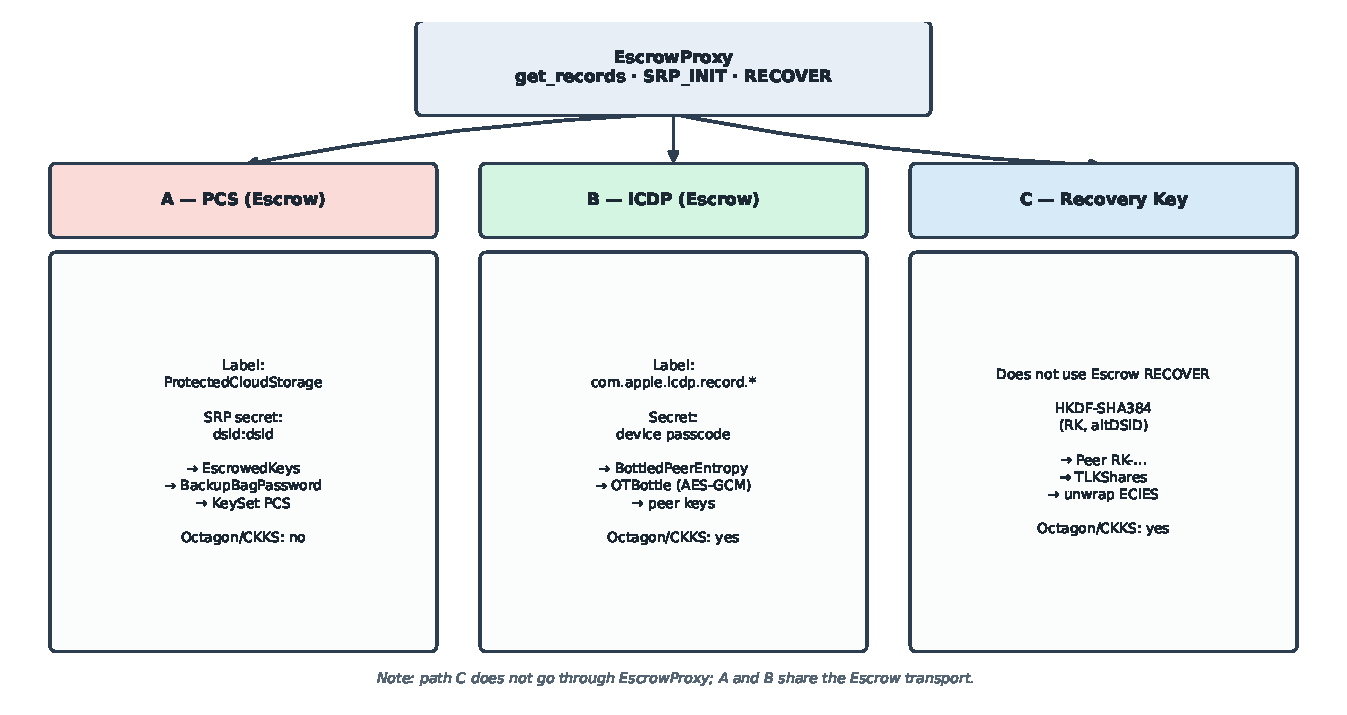
\includegraphics[keepaspectratio]{figures/fig02-escrow-porte.pdf}}

\textbf{Figure 2.} EscrowProxy as a shared transport for paths A and B;
path C does not use EscrowProxy.

This taxonomy is central: a large portion of integration errors arises
from treating the PCS Escrow path as if it provided access to Octagon.

\subsubsection{\texorpdfstring{6.3 Path A --- PCS Escrow
(\texttt{dsid:dsid})}{6.3 Path A --- PCS Escrow (dsid:dsid)}}\label{path-a-pcs-escrow-dsiddsid}

The SRP secret can be described as:

\begin{verbatim}
x = SHA256( salt ‖ SHA256( dsid ‖ ":" ‖ dsid ) )
\end{verbatim}

After \texttt{RECOVER} is obtained EscrowedKeys; the unwrap produces
BackupBagPassword, which is used to open the session's KeySet PCS. This
KeySet is sufficient for many backup scenarios without ADP based on
Manatee. It does not, alone, provide an Octagon peer identity nor the
TLKs of the current CKKS views.

\subsubsection{6.4 Path B --- iCDP (bottle
Octagon)}\label{path-b-icdp-bottle-octagon}

The \texttt{com.apple.icdp.record.*} records link Escrow to a device in
the Octagon domain (serial number, build, remaining HSM attempts).

\begin{itemize}
\tightlist
\item
  \textbf{Listing} (\texttt{get\_records}): non-destructive --- useful
  for forensic inventory.
\item
  \textbf{Recover} with passcode: each incorrect attempt consumes an HSM
  attempt (10 tries per record, in line with {[}8{]}). The IKE prototype
  requires explicit confirmation.
\item
  The correct passcode is the one in effect \textbf{at the time of
  record creation}, unless subsequently recreated (Sign out → Sign in on
  the device).
\item
  Output: EscrowBottle opened with \textbf{PBKDF2 + AES} →
  \textbf{BottledPeerEntropy} (\textasciitilde72 B) {[}19{]}.
\item
  Next step: Cuttlefish \texttt{fetchViableBottles} → \textbf{OTBottle
  Contents} → AES-GCM → peer keys (signing/encryption) and
  \texttt{peerId}.
\end{itemize}

\textbf{Orphan records:} metadata present, \texttt{Contents} absent or
zero-length → no peer keys; remain inventory evidence of
Escrow--Cuttlefish divergence.

\subsubsection{\texorpdfstring{6.5 Path C --- Recovery Key (without
Escrow
\texttt{RECOVER})}{6.5 Path C --- Recovery Key (without Escrow RECOVER)}}\label{path-c-recovery-key-without-escrow-recover}

When the passcode is unavailable (device lost, maximum attempts
exhausted, contents missing), the Recovery Key is used:

\begin{enumerate}
\def\labelenumi{\arabic{enumi}.}
\tightlist
\item
  \texttt{HKDF-SHA384} with IKM = UTF-8(RK) and salt = UTF-8(altDSID);
  distinct info strings for \emph{Recovery Signing Private Key} and
  \emph{Recovery Encryption Private Key}, yielding 56 bytes each
  {[}14{]}, {[}19{]}.
\item
  Map each 56-byte block to a P-384 private scalar via deterministic
  reduction \texttt{k\ =\ (entropy\_be\ mod\ (q−1))\ +\ 1}
  (TrustedPeersHelper / Day-11 evidence) {[}14{]}, {[}19{]}.
\item
  Peer ID = \texttt{RK-} + Base64(SHA-384 of the signing public key).
\item
  \texttt{ckAppInit} on the container
  \texttt{com.apple.security.keychain}.
\item
  \texttt{fetchRecoverableTLKShares} with \texttt{forPeer=RK-…}.
\item
  Unwrap ECIES of the shares → TLK per view → opening of CKKS views.
\end{enumerate}

An empty \texttt{forPeer} field can be used for inventorying encrypted
shares; unwrapping is possible only with the destination peer's keys.

\subsubsection{6.6 Typical Errors and
Diagnostics}\label{typical-errors-and-diagnostics}

{\def\LTcaptype{none} % do not increment counter
\begin{longtable}[]{@{}
  >{\raggedright\arraybackslash}p{(\linewidth - 2\tabcolsep) * \real{0.2727}}
  >{\raggedright\arraybackslash}p{(\linewidth - 2\tabcolsep) * \real{0.7273}}@{}}
\toprule\noalign{}
\begin{minipage}[b]{\linewidth}\raggedright
Symptom
\end{minipage} & \begin{minipage}[b]{\linewidth}\raggedright
Typical interpretation
\end{minipage} \\
\midrule\noalign{}
\endhead
\bottomrule\noalign{}
\endlastfoot
Credentials / M1 wrong (e.g.~codes type −6015) & Wrong SRP secret
(passcode vs \texttt{dsid:dsid} exchanged) \\
CLUBH / version header (e.g., −6122) & Version/header recovery
misaligned with the server \\
Listing OK, recover GCM fail & Entropy present but OTBottle contents
absent (orphan) \\
Recover succeeds, CKKS views are empty & Peer keys are incompatible with
the available TLKShares \\
RK lists share but unwrap=0 & Recovery Key does not match the binding /
peer error \\
\end{longtable}
}

Forensic diagnosis must record \textbf{which path} was being attempted:
without that context error codes become ambiguous.

\subsubsection{6.7 Secure Backup Variant with SMS
Challenge}\label{secure-backup-variant-with-sms-challenge}

A Secure Backup variant oriented to challenge SMS (observed as an
experimental option in the IKE prototype) exists. It does not alter the
taxonomy: it remains an additional Escrow mechanism on the
secret/challenge, not a substitute for Octagon. In this document, it is
treated as a marginal note: primary paths in the presence of ADP remain
iCDP or Recovery Key.

\subsubsection{6.8 Temporal flow and messages (reference Section
13.2)}\label{temporal-flow-and-messages-reference-section-13.2}

The EscrowProxy sequence diagram (\texttt{GETRECORDS} →
\texttt{SRP\_INIT} → \texttt{RECOVER}) and the example plist body are
presented in \textbf{Section 13.2} (Figure 7), reconstructed from
\texttt{EscrowProxyClient} / \texttt{EscrowSrpClient}.

\begin{center}\rule{0.5\linewidth}{0.5pt}\end{center}

\subsection{7. Octagon, Cuttlefish and opening of view
CKKS}\label{octagon-cuttlefish-and-opening-of-view-ckks}

\subsubsection{7.1 Octagon}\label{octagon}

\textbf{Octagon} designates the trust domain that connects devices, iCDP
records and Recovery Key for ADP, Manatee, and Keychain synchronization
{[}cf.~technical discussions on CKKS/Octagon; implementations in
{[}12{]}, {[}14{]}{]}. Without a peer identity capable of opening the
relevant views, the Manatee data for ADP-protected backup zones is
unavailable---although MMCS continues to serve ciphertext.

\subsubsection{7.2 Cuttlefish}\label{cuttlefish}

Service invoked via CloudKit on the container
\textbf{\texttt{com.apple.security.keychain}} (routing cuttlefish).
Relevant operations in this context:

\begin{itemize}
\tightlist
\item
  \texttt{fetchViableBottles} --- bottles and contents OTBottle;
\item
  \texttt{fetchRecoverableTLKShares} --- Recoverable TLK shares for
  peer.
\end{itemize}

\subsubsection{7.3 Opening of CKKS Views
(Steps)}\label{opening-of-ckks-views-steps}

\begin{enumerate}
\def\labelenumi{\arabic{enumi}.}
\tightlist
\item
  Open/synchronize the CKKS views of interest.
\item
  Identify \textbf{\texttt{tlkshare}} records; unwrap ECIES using the
  peer's encryption private key.
\item
  TLK persistence for view.
\item
  Unwrapping of \textbf{class keys} (\texttt{synckey}); decryption of
  items (\texttt{data}) along the CKKS path (AES-SIV / observed
  variants).
\item
  SecItem Interpretation (\texttt{agrp}, \texttt{class},
  \texttt{v\_Data}, \ldots) --- particularly relevant for Keychain
  experiments; for device backup, the PCS/Manatee-derived material takes
  precedence.
\end{enumerate}

Typically considered in the IKE prototype: \texttt{Manatee},
\texttt{Engram}, \texttt{ProtectedCloudStorage},
\texttt{LimitedPeersAllowed}, \texttt{Passwords}, \texttt{WiFi}.

\pandocbounded{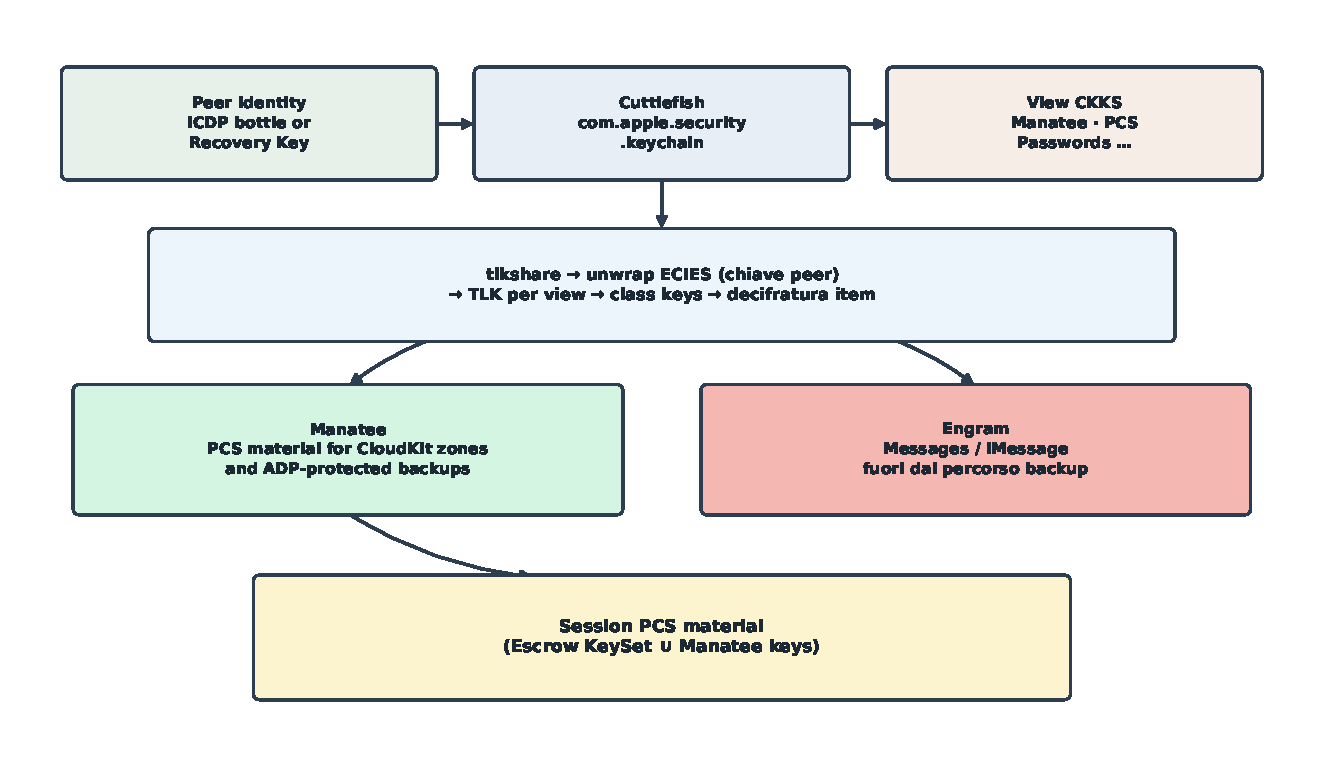
\includegraphics[keepaspectratio]{figures/fig03-octagon-ckks.pdf}}

\textbf{Figure 3.} From peer identity to PCS material: opening of CKKS
views; Manatee feeds the backup via ADP; Engram is excluded from this
pathway in the experiments described here.

\subsubsection{7.4 Temporal flow and messages (reference Section
13.3)}\label{temporal-flow-and-messages-reference-section-13.3}

The Cuttlefish/CKKS sequence diagram (Figure 8) and the
\texttt{ckAppInit} / \texttt{fetchRecoverableTLKShares} skeletons are in
\textbf{Section 13.3}, reconstructed by
\texttt{OctagonCuttlefishService} and \texttt{CkksVaultService}.

\begin{center}\rule{0.5\linewidth}{0.5pt}\end{center}

\subsection{8. Manatee, Engram, TLKShare, and Session PCS
Material}\label{manatee-engram-tlkshare-and-session-pcs-material}

{\def\LTcaptype{none} % do not increment counter
\begin{longtable}[]{@{}
  >{\raggedright\arraybackslash}p{(\linewidth - 2\tabcolsep) * \real{0.4348}}
  >{\raggedright\arraybackslash}p{(\linewidth - 2\tabcolsep) * \real{0.5652}}@{}}
\toprule\noalign{}
\begin{minipage}[b]{\linewidth}\raggedright
Concept
\end{minipage} & \begin{minipage}[b]{\linewidth}\raggedright
Description
\end{minipage} \\
\midrule\noalign{}
\endhead
\bottomrule\noalign{}
\endlastfoot
\textbf{TLK} & top-level key of a CKKS view \\
\textbf{TLKShare} & TLK wrapped ECIES toward a peer \\
\textbf{Manatee} & View CKKS observed as primary source of \textbf{PCS
material} for CloudKit zones / \textbf{backup with ADP} \\
\textbf{Engram} & Typically associated with Messages/iMessage {[}6{]};
not used as a PCS source in device backup experiments \\
\textbf{ProtectedCloudStorage} & Family of label/view PCS escrow and
vault \\
\textbf{Session PCS material} & Controlled union: Escrow KeySet
\textbf{or} (with ADP) Manatee keys \\
\end{longtable}
}

\textbf{Experimental observation.} The transfer of MMCS chunks with
incorrect PCS material results in objects that appear plausible but fail
MAC/digest checks. The dominant cause observed was not the network, but
rather the \textbf{IKM/incorrect PCS material} (Section 10).

\begin{center}\rule{0.5\linewidth}{0.5pt}\end{center}

\subsection{\texorpdfstring{9. CloudKit backup catalog
(\texttt{mbksync})}{9. CloudKit backup catalog (mbksync)}}\label{cloudkit-backup-catalog-mbksync}

Figure 4 shows the complete sequence from CloudKit inventory to MMCS
decryption (Sections 9--10).

\pandocbounded{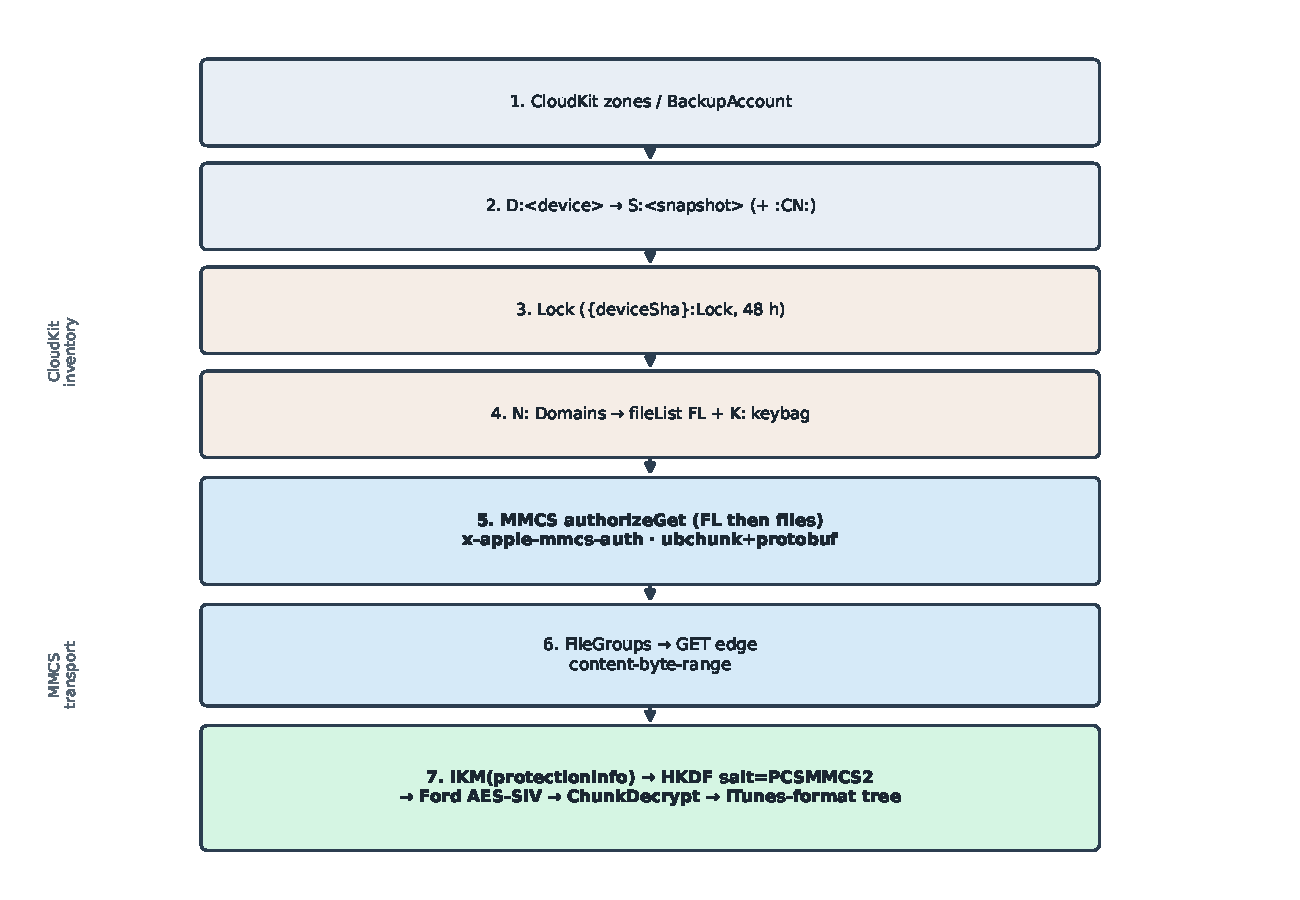
\includegraphics[keepaspectratio]{figures/fig04-mbksync-mmcs.pdf}}

\textbf{Figure 4.} Operation order: catalog/\texttt{Lock} (CloudKit),
then \texttt{authorizeGet}/Ford/\texttt{PCSMMCS2} (MMCS).

\subsubsection{9.1 Binding}\label{binding}

\begin{itemize}
\tightlist
\item
  Typical container: \textbf{\texttt{com.apple.backup.ios}}
\item
  Bundle: \textbf{\texttt{com.apple.backupd}}
\item
  Relevant zones: \texttt{\_defaultZone}, \textbf{\texttt{mbksync}}
\end{itemize}

Some zone/retrieve paths may fall back to the legacy Mobile Backup
Service host \texttt{\{partition\}-mobilebackup.icloud.com} (also
observed as \texttt{p32-mobilebackup.icloud.com}) with
\texttt{Accept:\ application/vnd.com.apple.mbs+protobuf} and
\texttt{X-Apple-MBS-Protocol-Version:\ 2.2} {[}19{]}. That transport is
a fallback, not a replacement for the CloudKit \texttt{mbksync} catalog
when the modern path is available.

\subsubsection{9.2 Record prefixes and
order}\label{record-prefixes-and-order}

Prefixes observed and treated as invariants:

{\def\LTcaptype{none} % do not increment counter
\begin{longtable}[]{@{}
  >{\raggedright\arraybackslash}p{(\linewidth - 2\tabcolsep) * \real{0.7083}}
  >{\raggedright\arraybackslash}p{(\linewidth - 2\tabcolsep) * \real{0.2917}}@{}}
\toprule\noalign{}
\begin{minipage}[b]{\linewidth}\raggedright
Prefix / name
\end{minipage} & \begin{minipage}[b]{\linewidth}\raggedright
Role
\end{minipage} \\
\midrule\noalign{}
\endhead
\bottomrule\noalign{}
\endlastfoot
\texttt{BackupAccount} & Account anchor \\
\texttt{D:} & Device \\
\texttt{S:} & Snapshot \\
\texttt{N:uuid:checksum=:0} & Domain catalog post-Lock (zone
\texttt{\_defaultZone}); holds the \texttt{fileList} CKAsset handle ---
\textbf{not} inline paths \\
\texttt{K:} & Keybag \\
\texttt{FL:\{sigHex\}} & Client-side synthetic id for a
Domain.\texttt{fileList} MMCS blob \\
\texttt{M:uuid:sig:0} & Classic manifest; field \texttt{files} lists
\texttt{F:} / \texttt{KA:} / \texttt{MA:} / \ldots{} \\
\texttt{KA:} / \texttt{MA:} / \texttt{LA:} / \texttt{NA:} / \texttt{JA:}
/ \ldots{} & Asset families
(e.g.~\texttt{MA:udid:uuid:checksumB64:size}) \\
\texttt{:CN:} / \texttt{CN:} & Contemporary checksum entries on
\texttt{S:} → drive \texttt{N:} record names \\
\end{longtable}
}

\textbf{Terminology note.} Laboratory dumps and some tooling comments
write \textbf{\texttt{EN:}}. On the wire the Domain record name is
\textbf{\texttt{N:…=:0}}. The leading \texttt{E} often comes from a
protobuf length byte (\texttt{0x45} =
\texttt{\textquotesingle{}E\textquotesingle{}}) preceding ASCII
\texttt{N:}; requesting a literal \texttt{EN:} record yields
\emph{Record not found}
(\texttt{CloudKitManifestChecksumParser.ToEnRecordName}) {[}19{]}.

\textbf{Catalog evolution.} Modern path: \texttt{S:\ →\ :CN:\ →\ N:}.
Classic path: \texttt{S:\ →\ M:\ →\ files} {[}19{]}. Clients that assume
only the classic list miss contemporary checksum/Domain records.

\textbf{Bootstrap order of restore} (not reorderable without loss of
state coherence):

\begin{verbatim}
zones → BackupAccount → D: → S: → (opt. MBS stub) → Lock → N: → K:
\end{verbatim}

\subsubsection{9.3 Lock}\label{lock}

\begin{itemize}
\tightlist
\item
  Typical Lock record: name \texttt{\{deviceSha\}:Lock}, type
  \texttt{Lock}, zone \texttt{mbksync}, owner = device SHA (without
  prefix \texttt{D:}), duration \textbf{172800} s (48 h) {[}19{]}.
\item
  Incorrect protobuf wrapping historically produced malformed Lock
  messages (e.g.~size class mismatches); the server failure string is
  \textbf{\texttt{Invalid\ lock\ id}} (MobileBackupServerExtension)
  {[}19{]}.
\item
  Tokens later used by MMCS carry metadata attributable to
  \textbf{Foreground Restore}.
\end{itemize}

\subsubsection{\texorpdfstring{9.4 \texttt{backupProperties} and
keybag}{9.4 backupProperties and keybag}}\label{backupproperties-and-keybag}

The snapshot field \textbf{\texttt{backupProperties}} is decrypted as
ShareProtection → \textbf{CUWK} with label \texttt{backupProperties} →
\textbf{PCSFP-GCM} with AAD type0 = field name {[}19{]}. Without session
PCS material it remains unreadable. In plaintext it feeds Lockdown.*
fields (UDID / model / serial) and sidecars (\texttt{Info.plist} /
\texttt{Manifest.plist}).

The keybag (\texttt{K:}) opens with PCS material (contemporary DER bag
or classic TLV; AES-KW where applicable). Only an open keybag
\textbf{and} Lock enable a semantically complete MMCS download.

\subsubsection{9.5 File lists: Domain retrieve, FL download, SQLite
inventory}\label{file-lists-domain-retrieve-fl-download-sqlite-inventory}

After Lock, the restore does \textbf{not} yet know Backup file paths.
Paths live inside per-domain \textbf{file-list blobs} referenced from
CloudKit \textbf{Domain} records. There are two nested meanings of
``file list'':

\begin{enumerate}
\def\labelenumi{\arabic{enumi}.}
\tightlist
\item
  \textbf{Domain catalog (\texttt{N:})} --- CloudKit metadata + an MMCS
  handle (\texttt{fileList} CKAsset).
\item
  \textbf{Decrypted SQLite flist (\texttt{flist\_*.db})} --- the real
  inventory (\texttt{Assets} ⋈ \texttt{FileMetadata}) that drives
  per-file \texttt{authorizeGet}.
\end{enumerate}

\paragraph{\texorpdfstring{9.5.1 From \texttt{:CN:} to Domain
\texttt{N:}}{9.5.1 From :CN: to Domain N:}}\label{from-cn-to-domain-n}

Modern snapshots expose \texttt{manifestChecksums} entries of the form
\texttt{:CN:uuid:checksum}. Each entry maps to a Domain record name
{[}19{]}:

\begin{verbatim}
N:{FILE_UUID}:{checksumBase64}=:0
\end{verbatim}

in zone \textbf{\texttt{\_defaultZone}}. The client batches
\texttt{record/retrieve} on those names (\texttt{BackupEnRecordService}
/ \texttt{DomainFileListParser}). Classic snapshots instead resolve
\texttt{manifestIDs} → \texttt{M:…:0} and read an inline \texttt{files}
field; the modern download path stays on \texttt{:CN:} / \texttt{N:}
when both eras coexist.

\paragraph{9.5.2 Domain record fields}\label{domain-record-fields}

A Domain record is a per-domain catalog. Observed fields include:

{\def\LTcaptype{none} % do not increment counter
\begin{longtable}[]{@{}
  >{\raggedright\arraybackslash}p{(\linewidth - 2\tabcolsep) * \real{0.5385}}
  >{\raggedright\arraybackslash}p{(\linewidth - 2\tabcolsep) * \real{0.4615}}@{}}
\toprule\noalign{}
\begin{minipage}[b]{\linewidth}\raggedright
Field
\end{minipage} & \begin{minipage}[b]{\linewidth}\raggedright
Role
\end{minipage} \\
\midrule\noalign{}
\endhead
\bottomrule\noalign{}
\endlastfoot
\texttt{domainName} / \texttt{domain} & Domain identity (\texttt{domain}
may be PCS-encrypted on the wire) \\
\texttt{version} & Domain version \\
\texttt{cumulativeFileCount} / \texttt{Directory} / \texttt{Asset} /
\texttt{EmptyFile} / \texttt{SymLink} & Counts \\
\texttt{fileListEncoding} & \textbf{\texttt{2}} = after MMCS (+ optional
LZFSE) the blob is \textbf{SQLite} (\texttt{SQLite\ format\ 3}), not
protobuf \\
\texttt{fileList} & CKAsset / MMCS descriptor (signature, size, auth,
ContentBaseUrl, protection wrap) \\
\texttt{newAssets} / \texttt{deletedAssets} & Optional asset-name
deltas \\
\end{longtable}
}

Optional PCS field decrypt (\texttt{DomainPcsFieldDecryptor}) uses
zone/record ShareProtection and \textbf{PCS GCM} (\texttt{PcsGcmDataA})
with AAD = UTF-8 field name. On many modern captures \texttt{fileList}
is already a plaintext CKAsset handle; brute PCS over that field is
skipped when the MMCS auth is already present.

The MMCS descriptor extracted from \texttt{fileList} yields a synthetic
client asset \texttt{FL:\{signatureHex\}} with
\texttt{x-apple-mmcs-auth} of the form
\texttt{\{sig21hex\}\ \{token17hex\}\ \{CAog…\}}
(\texttt{DomainFileListParser.FileListAsset}).

\paragraph{9.5.3 Download and decrypt the FL
blob}\label{download-and-decrypt-the-fl-blob}

Each Domain.\texttt{fileList} is downloaded with the same MMCS pipeline
as backup files (Section 10):

\begin{verbatim}
x-apple-mmcs-auth(FL) → authorizeGet → FileGroups → content-byte-range
  → IKM from contents.protectionInfo (NISTKDF "wrapping key wrap me" + AES-KW)
  → Ford / PCSMMCS2 (or MMCS-CFB when applicable)
  → optional LZFSE (magic bvx*) → SQLite format 3
\end{verbatim}

The decrypted database is materialized as \texttt{flist\_\{sig\}.db}.
\textbf{\texttt{fileListEncoding\ =\ 2}} is the invariant that the
expanded payload is SQLite (\texttt{Assets} / \texttt{FileMetadata}),
not a protobuf inventory {[}19{]}.

\paragraph{9.5.4 Reading the SQLite
inventory}\label{reading-the-sqlite-inventory}

\texttt{FileListSqliteParser} joins:

\begin{Shaded}
\begin{Highlighting}[]
\KeywordTok{SELECT}\NormalTok{ a.recordIDSuffix, a.encryptionKey, a.assetSignature, a.assetSize, …}
\NormalTok{       f.relativePath, f.}\KeywordTok{size}\NormalTok{, f.}\KeywordTok{mode}\NormalTok{, f.protectionClass, f.modified, f.birth, …}
\KeywordTok{FROM}\NormalTok{ Assets a}
\KeywordTok{JOIN}\NormalTok{ FileMetadata f }\KeywordTok{ON}\NormalTok{ a.inode }\OperatorTok{=}\NormalTok{ f.inode}
\end{Highlighting}
\end{Shaded}

{\def\LTcaptype{none} % do not increment counter
\begin{longtable}[]{@{}
  >{\raggedright\arraybackslash}p{(\linewidth - 2\tabcolsep) * \real{0.6000}}
  >{\raggedright\arraybackslash}p{(\linewidth - 2\tabcolsep) * \real{0.4000}}@{}}
\toprule\noalign{}
\begin{minipage}[b]{\linewidth}\raggedright
Column / derived field
\end{minipage} & \begin{minipage}[b]{\linewidth}\raggedright
Use downstream
\end{minipage} \\
\midrule\noalign{}
\endhead
\bottomrule\noalign{}
\endlastfoot
\texttt{recordIDSuffix} & CloudKit / MMCS rid
(\texttt{uuid:token=:size}) → \texttt{F:…} / PrivilegedBatch seed \\
\texttt{assetSignature} (21 B) & authorizeGet \textbf{f1} \\
\texttt{encryptionKey} & per-file class-key / AES material ---
\textbf{not} Ford IKM \\
\texttt{relativePath}, \texttt{mode}, \texttt{protectionClass}, times,
uid/gid & inventory / Manifest sidecars \\
\texttt{fileID} & \texttt{SHA1(domain\ +\ "-"\ +\ relativePath)} for the
iTunes \texttt{Backup/} tree \\
\end{longtable}
}

Directories, symlinks, empty-file stubs, missing 21-B signatures, and
zero-size rows are skipped by the download planner
(\texttt{FlistDownloadPlanBuilder}). A full inventory join (including
directories) feeds \texttt{ManifestFromFileListBuilder} when rebuilding
\texttt{Manifest.db} from flists.

\paragraph{9.5.5 From flist rows to Backup
files}\label{from-flist-rows-to-backup-files}

For each Domain, the interleaved restore does:

\begin{enumerate}
\def\labelenumi{\arabic{enumi}.}
\tightlist
\item
  Download / decrypt / parse that Domain's FL.
\item
  Build a batch of \texttt{BackupAsset} rows from the SQLite join.
\item
  Ensure \texttt{x-apple-mmcs-auth} per file (often via PrivilegedBatch
  / PreAuth join on \texttt{A:} / \texttt{KA:} / \texttt{MA:} when the
  flist row has no auth).
\item
  Batch \texttt{authorizeGet} (typically ≤ 12 files) with \textbf{f1} =
  \texttt{assetSignature}, \textbf{f2} = CAog, \textbf{f4} = companion
  token {[}24{]}.
\item
  Edge GET → Ford/\texttt{PCSMMCS2} (or MMCS-CFB) → write
  \texttt{Backup/\{fileID{[}0..2{]}\}/\{fileID\}}.
\item
  Keep a \textbf{per-domain} MMCS assembly session (Section 10.5).
\end{enumerate}

Only after flists are expanded does the client know which MMCS objects
belong in the Backup tree. Counting Domain records or raw CloudKit
assets is \textbf{not} a substitute for the flist inventory.

\subsubsection{9.6 Temporal flow and messages (reference Sections
13.4--13.6)}\label{temporal-flow-and-messages-reference-sections-13.413.6}

The CloudKit inventory sequence (Figure 9) and the dedicated file-list
sequence (Figure 11) are in \textbf{Sections 13.4 and 13.6},
reconstructed from \texttt{CloudKitAssetService},
\texttt{BackupEnRecordService}, \texttt{DomainFileListParser},
\texttt{FileListSqliteParser}, and \texttt{BackupDownloadService}.

\begin{center}\rule{0.5\linewidth}{0.5pt}\end{center}

\subsection{10. MMCS: authorizeGet, FileGroups, Ford and
PCSMMCS2}\label{mmcs-authorizeget-filegroups-ford-and-pcsmmcs2}

\subsubsection{10.1 Role}\label{role}

\textbf{MMCS} (\emph{MobileMe Cloud Storage}, historical nomenclature
persisting in the protocol) delivers the bytes of assets; CloudKit
maintains the inventory. The critical conversation is:

\begin{verbatim}
x-apple-mmcs-auth  →  POST {contentHost}/{dsid}/authorizeGet
  MIME: application/vnd.com.apple.me.ubchunk+protobuf
  → FileGroups (host template + ChunkInfo + assembly refs)
  → GET edge ?content-byte-range=start-end
\end{verbatim}

Typical hosts: \texttt{\{partition\}-content.icloud.com} or
ContentBaseUrl per-record. The use of \texttt{authorizeGet} and chunking
toward third-party storage has already been documented in the 2013
disclosures {[}4{]}, {[}5{]}; this work updates the association with the
CloudKit catalog \texttt{mbksync} and the derivation \texttt{PCSMMCS2}.

\subsubsection{\texorpdfstring{10.2 Header
\texttt{x-apple-mmcs-auth}}{10.2 Header x-apple-mmcs-auth}}\label{header-x-apple-mmcs-auth}

Observed outer shape: \texttt{\{hex21\}\ \{hex21\}\ \{CAog…\}}
(base64url blob with Foreground Restore marker) {[}19{]}. In the
authorizeGet ubchunk \textbf{per-file} entry, field roles are {[}24{]}:

{\def\LTcaptype{none} % do not increment counter
\begin{longtable}[]{@{}
  >{\raggedright\arraybackslash}p{(\linewidth - 2\tabcolsep) * \real{0.5385}}
  >{\raggedright\arraybackslash}p{(\linewidth - 2\tabcolsep) * \real{0.4615}}@{}}
\toprule\noalign{}
\begin{minipage}[b]{\linewidth}\raggedright
Field
\end{minipage} & \begin{minipage}[b]{\linewidth}\raggedright
Role
\end{minipage} \\
\midrule\noalign{}
\endhead
\bottomrule\noalign{}
\endlastfoot
\textbf{f1} & Assets \texttt{assetSignature} verbatim (21 B, typically
\texttt{0x04‖20B}) \\
\textbf{f2} & \texttt{CAog…} token string \\
\textbf{f4} & Companion typically \texttt{0x01‖20B} \\
\end{longtable}
}

Batch-header rebuild from entry{[}0{]} uses
\texttt{hex(f1)\ +\ hex(f4)\ +\ ascii(f2)}. Using a CloudKit mmcs-auth
fragment as \textbf{f1} yields plans that look authorized and then fail
at the edge {[}19{]}, {[}24{]}.

\subsubsection{10.3 FileGroups and the dual nature of the
object}\label{filegroups-and-the-dual-nature-of-the-object}

Each FileGroup maps to a GET host and contains nested ChunkInfo
(checksums of 21 or 45 B, \texttt{chunkEncryptionKey}, \texttt{ctLen},
offset, assembly references). \textbf{The same edge object} may expose:

\begin{itemize}
\tightlist
\item
  \textbf{Ford} material (keys) at offset 0 --- terminology already
  present in {[}6{]};
\item
  \textbf{ChunkInfo} data at other ranges.
\end{itemize}

Confusion between the two yields MAC failures that look like partial
success. Day-11 evidence further bounds Ford \texttt{ctLen} (practical
window starting at \texttt{0x12}) and describes data-ChunkInfo staging
(header length \texttt{0x28}; LE u64 at \texttt{hdr{[}0x20{]}} = wire
data length; MAC over the trailing 20 bytes of the 21-B checksum)
{[}19{]}.

\subsubsection{\texorpdfstring{10.4 IKM and Ford KDF
(\texttt{PCSMMCS2})}{10.4 IKM and Ford KDF (PCSMMCS2)}}\label{ikm-and-ford-kdf-pcsmmcs2}

The IKM is \textbf{not} the file-list \texttt{EncryptionKey}. On owned
CloudKit records it is obtained by unwrapping
\texttt{contents.protectionInfo} with the zone master via
\textbf{AES-KW} after \textbf{NISTKDF} with label
\textbf{\texttt{wrapping\ key\ wrap\ me}} {[}19{]}, {[}25{]}:

\begin{verbatim}
IKM = AES-KW( NISTKDF(zoneMaster, "wrapping key wrap me"), protectionInfoWrap )
\end{verbatim}

Then:

\begin{verbatim}
HKDF-SHA256(
  ikm  = fileKey,       // from protectionInfo unwrap
  salt = "PCSMMCS2",
  info = "",
  len  = 64             // 0x40
)
\end{verbatim}

Typical Ford layout: \texttt{lead(1)\ ‖\ nonce(16)\ ‖\ body}, with body
= \texttt{tag(16)\ ‖\ ciphertext} at offset \texttt{0x11}. Decryption
uses \textbf{AES-SIV (RFC 5297)} with AD \texttt{{[}nonce,\ lead{]}}.
Per-chunk expansion uses HKDF info \texttt{signature-key} (0x60 B →
k1/k2/k3).

\subsubsection{10.5 Classifiers, cache, and per-domain
sessions}\label{classifiers-cache-and-per-domain-sessions}

\begin{itemize}
\tightlist
\item
  Lead \texttt{0x04} typical for Ford ciphertext at offset 0.
\item
  Valid data chunks may begin with \textbf{\texttt{0xC4}} (and other
  leads ≠ \texttt{0x04}); treating them as invalid Ford was a
  classification error that blocked otherwise complete downloads.
\item
  Ownership descriptors of 45 B with prefix \texttt{0C\ 0F\ 01\ 04} ≠
  data checksums of 21 B.
\item
  Local cache keyed by hex signature; do not store Ford blobs without
  IKM (cache corruption).
\item
  Stable fill order: authorizeGet → FileGroups → ranged GET → open Ford
  → fill chunks → ChunkDecrypt with VerifyDigest.
\item
  \textbf{Per-domain isolation:} domains may run in parallel, but each
  keeps its own assembly / FileGroup cache shard --- sharing one
  assembly session across domains is an anti-pattern (Section 10.7)
  {[}19{]}.
\end{itemize}

\subsubsection{10.6 Incomplete plans and batch
pre-authorization}\label{incomplete-plans-and-batch-pre-authorization}

An authorized GET plan is \textbf{incomplete} (and must be treated as a
failure) if URL chunks, edge signatures, or the sum of byte ranges is
less than the declared size. Estimating missing ranges is the fastest
path to cache corruption.

At the upper level, the client organizes batch pre-authorization waves:
it prepares signatures and tokens for multiple assets, refreshes
Anisette if the edge rejects the identity, and only then issues an
authorizeGet. Scalability (thousands of files) does not alter the
semantics: each FileGroup remains a local contract among signature,
range, and decryption stages.

\subsubsection{10.7 Anti-pattern MMCS}\label{anti-pattern-mmcs}

\begin{enumerate}
\def\labelenumi{\arabic{enumi}.}
\tightlist
\item
  Use the EncryptionKey from the file list as IKM Ford.
\item
  Store in cache every blob with lead \texttt{0x04} without opening it
  with IKM.
\item
  Treat 45 B descriptors as 21 B data checksums.
\item
  Reverse the filling order (decrypt the data before opening Ford).
\item
  Share a single assembly session among FileGroups from different
  domains.
\item
  Reconstruct \texttt{x-apple-mmcs-auth} by swapping the signature/token
  fields.
\end{enumerate}

Each anti-pattern was observed as a silent failure or as a misleading
partial success during the 2026 experiments.

\subsubsection{10.8 Temporal flow and messages (reference Section
13.5)}\label{temporal-flow-and-messages-reference-section-13.5}

The UML detail of \texttt{authorizeGet} and of GET
\texttt{content-byte-range} (Figure 10), including headers and MIME, is
in \textbf{Section 13.5}, reconstructed by
\texttt{BackupDownloadService} / \texttt{UbChunkBuilder}.

\begin{center}\rule{0.5\linewidth}{0.5pt}\end{center}

\subsection{11. Forensic Materialization and
Verification}\label{forensic-materialization-and-verification}

Output objective: an \textbf{iTunes-compatible tree} {[}19{]}:

\begin{itemize}
\tightlist
\item
  hashed path \texttt{Backup/\{fileID{[}0..2{]}\}/\{fileID\}} with
  \texttt{fileID} = SHA1 hex of the content blob as laid out by the
  restore;
\item
  Manifest rows keyed consistently with
  \texttt{SHA1(domain\ +\ "-"\ +\ relativePath)} where applicable;
\item
  \texttt{Manifest.db} from decrypted \texttt{MA:} (and related)
  candidates;
\item
  sidecars \texttt{Info.plist}, \texttt{Status.plist},
  \texttt{Manifest.plist} (preferably aligned with plaintext
  \texttt{backupProperties});
\item
  optional tree nesting
  \texttt{\{root\}/\{udid\}/{[}\{snapshotGuid\}{]}{[}\{timestamp\}{]}/}.
\end{itemize}

Forensic verification does not stop at download completion: it includes
file counts, digests, comparison with the \texttt{N:}/\texttt{EN:}
inventory, and awareness of \textbf{orphans} (catalog name, no MMCS
asset) and of payloads that are \textbf{not} Ford/MMCS crypto (e.g.~some
third-party model files observed in lab captures) {[}19{]}. Domains must
keep separate MMCS assembly state (Section 10.5).

\begin{center}\rule{0.5\linewidth}{0.5pt}\end{center}

\subsection{12. Synthesis of pathways, operational risks, and
limitations}\label{synthesis-of-pathways-operational-risks-and-limitations}

\subsubsection{12.1 Three paths → PCS
material}\label{three-paths-pcs-material}

{\def\LTcaptype{none} % do not increment counter
\begin{longtable}[]{@{}
  >{\raggedright\arraybackslash}p{(\linewidth - 4\tabcolsep) * \real{0.2439}}
  >{\raggedright\arraybackslash}p{(\linewidth - 4\tabcolsep) * \real{0.2439}}
  >{\raggedright\arraybackslash}p{(\linewidth - 4\tabcolsep) * \real{0.5122}}@{}}
\toprule\noalign{}
\begin{minipage}[b]{\linewidth}\raggedright
Path
\end{minipage} & \begin{minipage}[b]{\linewidth}\raggedright
Input
\end{minipage} & \begin{minipage}[b]{\linewidth}\raggedright
Output toward backup
\end{minipage} \\
\midrule\noalign{}
\endhead
\bottomrule\noalign{}
\endlastfoot
\textbf{A --- PCS Escrow} & Escrow \texttt{dsid:dsid} & EscrowedKeys /
BackupBagPassword → KeySet \\
\textbf{B --- iCDP} & Escrow passcode + OTBottle & Peer → view CKKS →
Manatee/PCS \\
\textbf{C --- Recovery Key} & HKDF RK + TLKShares & TLK → view CKKS →
Manatee/PCS \\
\end{longtable}
}

\pandocbounded{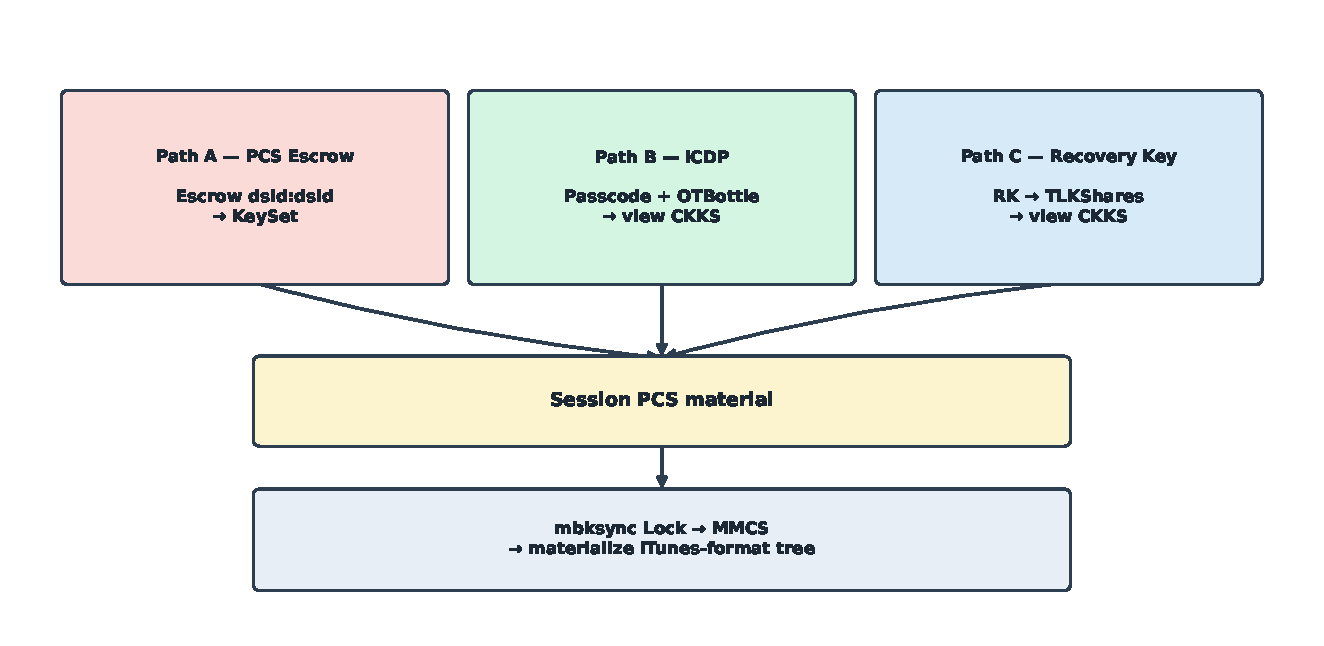
\includegraphics[keepaspectratio]{figures/fig05-tre-cammini.pdf}}

\textbf{Figure 5.} A/B/C convergence on the PCS material, followed by
the \texttt{mbksync}/MMCS sequence.

With ADP enabled, either B or C are typically required; A alone is often
insufficient.

\subsubsection{12.2 Operational Risks}\label{operational-risks}

\begin{enumerate}
\def\labelenumi{\arabic{enumi}.}
\tightlist
\item
  Anisette remint mid-SRP, or MidService/\texttt{MD-M} identity mismatch
  vs CPD (\texttt{ec=-22410} on complete) {[}23{]}.
\item
  Confusion between web PET / idmsa sessions and native AuthKit
  sessions.
\item
  Brute force against HSM attempt limits on Escrow records.
\item
  Current credentials applied to records created under previous
  credentials.
\item
  IKM taken from the file-list EncryptionKey instead of
  \texttt{protectionInfo} unwrap (NISTKDF / AES-KW).
\item
  Ford/ChunkInfo cache corruption; shared assembly across domains.
\item
  Expired tokens after prolonged Escrow operations (refresh required).
\item
  Treating ADP failure as ``old iOS only'': laboratory captures showed
  commercial clients able to talk to recent backup eras yet still
  receiving \textbf{HTTP 403} when ADP gated the crypto path {[}19{]}.
\end{enumerate}

\subsubsection{12.3 Declared Limits}\label{declared-limits}

\begin{itemize}
\tightlist
\item
  Apple's private surfaces do not constitute a stable contract.
\item
  Not every historical file is recoverable (orphans, non-MMCS payloads,
  third-party encryption).
\item
  Emulated Anisette is not indefinitely usable; Mac-provisioned identity
  ≠ \texttt{akd} identity.
\item
  Opening Keychain via CKKS in the IKE prototype is an experimental
  path, not a complete Keychain product.
\item
  This document does not cover services outside the defined scope
  (Section 1.3).
\end{itemize}

\begin{center}\rule{0.5\linewidth}{0.5pt}\end{center}

\subsection{13. Temporal UML Flows and Protocol
Messages}\label{temporal-uml-flows-and-protocol-messages}

This section consolidates the \textbf{sequence diagrams} (UML style) and
the \textbf{message skeletons} reconstructed from the independent IKE
implementation (\texttt{src/iCloudKitExtractor.Core}). Sensitive values
are replaced with placeholders
\texttt{\textless{}REDACTED\textgreater{}}; field structures, endpoints,
and call orders match the cited code.

\textbf{Conventions:} Blue arrows = client→server requests; green arrows
= responses; beige boxes = local processing. Host \texttt{pXX-} = iCloud
session partition.

\subsubsection{13.1 GrandSlam / GsService2}\label{grandslam-gsservice2}

\textbf{Prelude (MidService).} Before GsService2 init/complete, real
\texttt{akd} clients run MidService provisioning (\texttt{lookup} →
\texttt{startMachineProvisioning} / \texttt{spim} →
\texttt{finishMachineProvisioning} / \texttt{ptm} / \texttt{tk}) as in
Section 4.1 and {[}22{]} (\texttt{AdiProvisioningService}).

\textbf{Sources:} \texttt{Services/Auth/GsaGrandSlamAuthService.cs},
\texttt{GsaSrpClient.cs}, \texttt{GrandSlamCpdBuilder.cs},
\texttt{AdiProvisioningService.cs}.

\pandocbounded{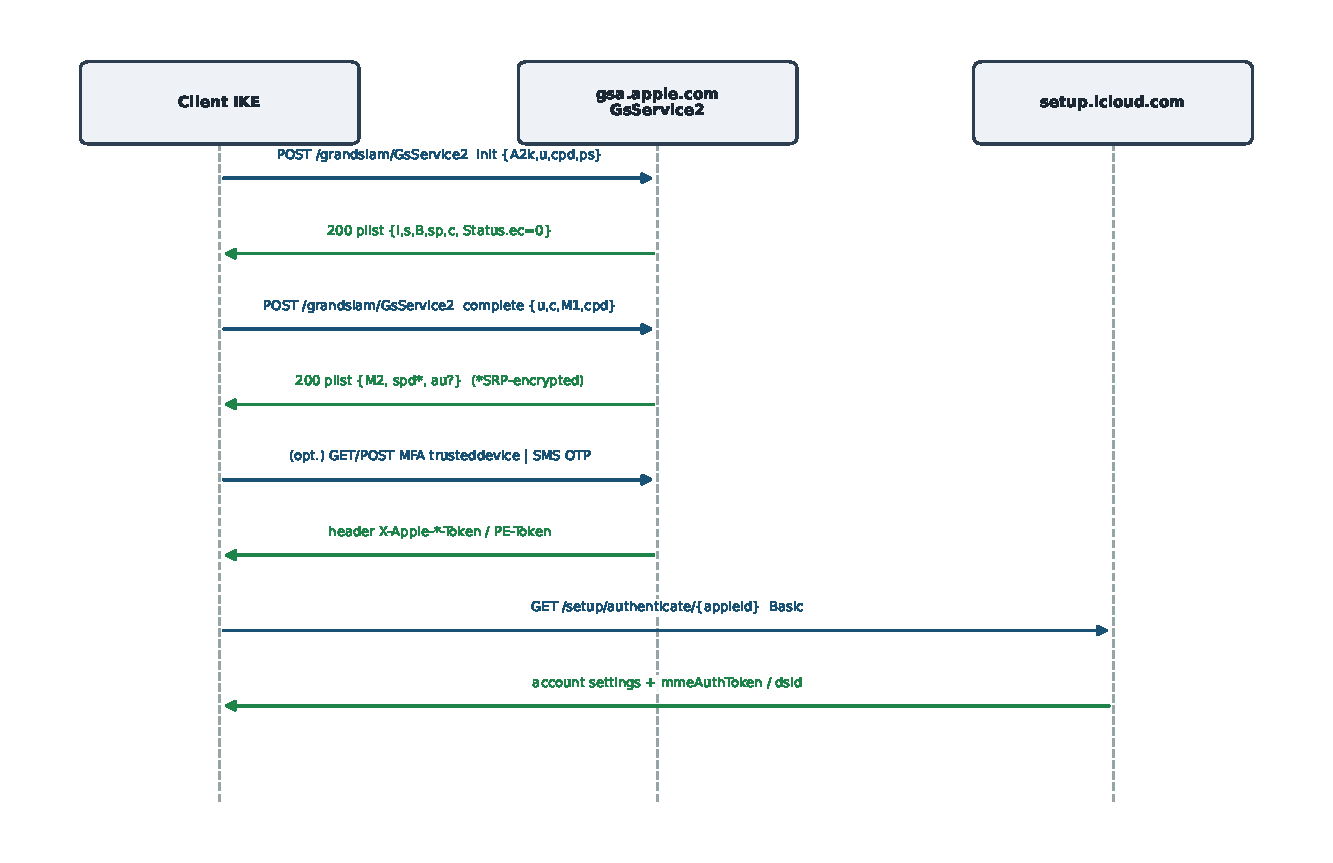
\includegraphics[keepaspectratio]{figures/fig06-seq-grandslam.pdf}}

\textbf{Figure 6.} GrandSlam Sequence: init/complete SRP, optional MFA,
session materialization on \texttt{setup.icloud.com}.

\textbf{Request --- GsService2 init}
(\texttt{POST\ https://gsa.apple.com/grandslam/GsService2},
\texttt{Content-Type:\ text/x-xml-plist}):

\begin{Shaded}
\begin{Highlighting}[]
\CommentTok{\textless{}!{-}{-} scheletro; Header/Request wrappati da BuildGsService2Request("init", …) {-}{-}\textgreater{}}
\NormalTok{\textless{}}\KeywordTok{dict}\NormalTok{\textgreater{}}
\NormalTok{  \textless{}}\KeywordTok{key}\NormalTok{\textgreater{}A2k\textless{}/}\KeywordTok{key}\NormalTok{\textgreater{} \textless{}}\KeywordTok{data}\NormalTok{\textgreater{}}\CommentTok{\textless{}!{-}{-} SRP public A, 256 B {-}{-}\textgreater{}}\NormalTok{\textless{}/}\KeywordTok{data}\NormalTok{\textgreater{}}
\NormalTok{  \textless{}}\KeywordTok{key}\NormalTok{\textgreater{}u\textless{}/}\KeywordTok{key}\NormalTok{\textgreater{}   \textless{}}\KeywordTok{string}\NormalTok{\textgreater{}user@example.com\textless{}/}\KeywordTok{string}\NormalTok{\textgreater{}}
\NormalTok{  \textless{}}\KeywordTok{key}\NormalTok{\textgreater{}cpd\textless{}/}\KeywordTok{key}\NormalTok{\textgreater{} \textless{}}\KeywordTok{dict}\NormalTok{\textgreater{}}
    \CommentTok{\textless{}!{-}{-} Client{-}Time, X{-}Apple{-}I{-}MD*, Mme{-}Device{-}Id, bootstrap, svct=iCloud, … {-}{-}\textgreater{}}
\NormalTok{  \textless{}/}\KeywordTok{dict}\NormalTok{\textgreater{}}
\NormalTok{  \textless{}}\KeywordTok{key}\NormalTok{\textgreater{}ps\textless{}/}\KeywordTok{key}\NormalTok{\textgreater{}  \textless{}}\KeywordTok{array}\NormalTok{\textgreater{}\textless{}}\KeywordTok{string}\NormalTok{\textgreater{}s2k\textless{}/}\KeywordTok{string}\NormalTok{\textgreater{}\textless{}}\KeywordTok{string}\NormalTok{\textgreater{}s2k\_fo\textless{}/}\KeywordTok{string}\NormalTok{\textgreater{}\textless{}/}\KeywordTok{array}\NormalTok{\textgreater{}}
\NormalTok{\textless{}/}\KeywordTok{dict}\NormalTok{\textgreater{}}
\end{Highlighting}
\end{Shaded}

Typical headers (beyond Anisette \texttt{X-Apple-I-MD*}): AuthKit iPhone
or AuthKit Windows profile.

\textbf{Response --- init} (ec=0):

\begin{Shaded}
\begin{Highlighting}[]
\NormalTok{\textless{}}\KeywordTok{dict}\NormalTok{\textgreater{}}
\NormalTok{  \textless{}}\KeywordTok{key}\NormalTok{\textgreater{}Status\textless{}/}\KeywordTok{key}\NormalTok{\textgreater{} \textless{}}\KeywordTok{dict}\NormalTok{\textgreater{}\textless{}}\KeywordTok{key}\NormalTok{\textgreater{}ec\textless{}/}\KeywordTok{key}\NormalTok{\textgreater{}\textless{}}\KeywordTok{integer}\NormalTok{\textgreater{}0\textless{}/}\KeywordTok{integer}\NormalTok{\textgreater{}\textless{}/}\KeywordTok{dict}\NormalTok{\textgreater{}}
\NormalTok{  \textless{}}\KeywordTok{key}\NormalTok{\textgreater{}i\textless{}/}\KeywordTok{key}\NormalTok{\textgreater{}  \textless{}}\KeywordTok{integer}\NormalTok{\textgreater{}20016\textless{}/}\KeywordTok{integer}\NormalTok{\textgreater{}   }\CommentTok{\textless{}!{-}{-} iterazioni; default IKE se assente {-}{-}\textgreater{}}
\NormalTok{  \textless{}}\KeywordTok{key}\NormalTok{\textgreater{}s\textless{}/}\KeywordTok{key}\NormalTok{\textgreater{}  \textless{}}\KeywordTok{data}\NormalTok{\textgreater{}}\CommentTok{\textless{}!{-}{-} salt {-}{-}\textgreater{}}\NormalTok{\textless{}/}\KeywordTok{data}\NormalTok{\textgreater{}}
\NormalTok{  \textless{}}\KeywordTok{key}\NormalTok{\textgreater{}B\textless{}/}\KeywordTok{key}\NormalTok{\textgreater{}  \textless{}}\KeywordTok{data}\NormalTok{\textgreater{}}\CommentTok{\textless{}!{-}{-} SRP public B {-}{-}\textgreater{}}\NormalTok{\textless{}/}\KeywordTok{data}\NormalTok{\textgreater{}}
\NormalTok{  \textless{}}\KeywordTok{key}\NormalTok{\textgreater{}sp\textless{}/}\KeywordTok{key}\NormalTok{\textgreater{} \textless{}}\KeywordTok{string}\NormalTok{\textgreater{}s2k\textless{}/}\KeywordTok{string}\NormalTok{\textgreater{}}
\NormalTok{  \textless{}}\KeywordTok{key}\NormalTok{\textgreater{}c\textless{}/}\KeywordTok{key}\NormalTok{\textgreater{}  \textless{}}\KeywordTok{string}\NormalTok{\textgreater{}}\CommentTok{\textless{}!{-}{-} challenge {-}{-}\textgreater{}}\NormalTok{\textless{}/}\KeywordTok{string}\NormalTok{\textgreater{}}
\NormalTok{\textless{}/}\KeywordTok{dict}\NormalTok{\textgreater{}}
\end{Highlighting}
\end{Shaded}

\textbf{Request --- complete} (same CPD as init; \textbf{do not} send
\texttt{M2} in the body):

\begin{Shaded}
\begin{Highlighting}[]
\NormalTok{\textless{}}\KeywordTok{dict}\NormalTok{\textgreater{}}
\NormalTok{  \textless{}}\KeywordTok{key}\NormalTok{\textgreater{}u\textless{}/}\KeywordTok{key}\NormalTok{\textgreater{}  \textless{}}\KeywordTok{string}\NormalTok{\textgreater{}user@example.com\textless{}/}\KeywordTok{string}\NormalTok{\textgreater{}}
\NormalTok{  \textless{}}\KeywordTok{key}\NormalTok{\textgreater{}c\textless{}/}\KeywordTok{key}\NormalTok{\textgreater{}  \textless{}}\KeywordTok{string}\NormalTok{\textgreater{}}\CommentTok{\textless{}!{-}{-} challenge da init {-}{-}\textgreater{}}\NormalTok{\textless{}/}\KeywordTok{string}\NormalTok{\textgreater{}}
\NormalTok{  \textless{}}\KeywordTok{key}\NormalTok{\textgreater{}M1\textless{}/}\KeywordTok{key}\NormalTok{\textgreater{} \textless{}}\KeywordTok{data}\NormalTok{\textgreater{}}\CommentTok{\textless{}!{-}{-} prova client SRP {-}{-}\textgreater{}}\NormalTok{\textless{}/}\KeywordTok{data}\NormalTok{\textgreater{}}
\NormalTok{  \textless{}}\KeywordTok{key}\NormalTok{\textgreater{}cpd\textless{}/}\KeywordTok{key}\NormalTok{\textgreater{}\textless{}}\KeywordTok{dict}\NormalTok{\textgreater{}}\CommentTok{\textless{}!{-}{-} identico a init {-}{-}\textgreater{}}\NormalTok{\textless{}/}\KeywordTok{dict}\NormalTok{\textgreater{}}
\NormalTok{\textless{}/}\KeywordTok{dict}\NormalTok{\textgreater{}}
\end{Highlighting}
\end{Shaded}

\textbf{Response --- complete:} \texttt{M2} (server verification),
\texttt{spd} (encrypted SRP blob → adsid, GsIdmsToken,
\texttt{com.apple.gs.idms.pet}, \ldots), optional
\texttt{au=trustedDeviceSecondaryAuth}.

\textbf{Typical post-login request:}
\texttt{GET\ https://setup.icloud.com/setup/authenticate/\{appleId\}}
with Basic → \texttt{dsid}, \texttt{mmeAuthToken}, partition URL.

\begin{center}\rule{0.5\linewidth}{0.5pt}\end{center}

\subsubsection{\texorpdfstring{13.2 EscrowProxy (\texttt{GETRECORDS} →
\texttt{SRP\_INIT} →
\texttt{RECOVER})}{13.2 EscrowProxy (GETRECORDS → SRP\_INIT → RECOVER)}}\label{escrowproxy-getrecords-srp_init-recover}

\textbf{Sources:} \texttt{Services/Escrow/EscrowProxyClient.cs},
\texttt{EscrowSrpClient.cs}, \texttt{EscrowRecoveryService.cs}.

\pandocbounded{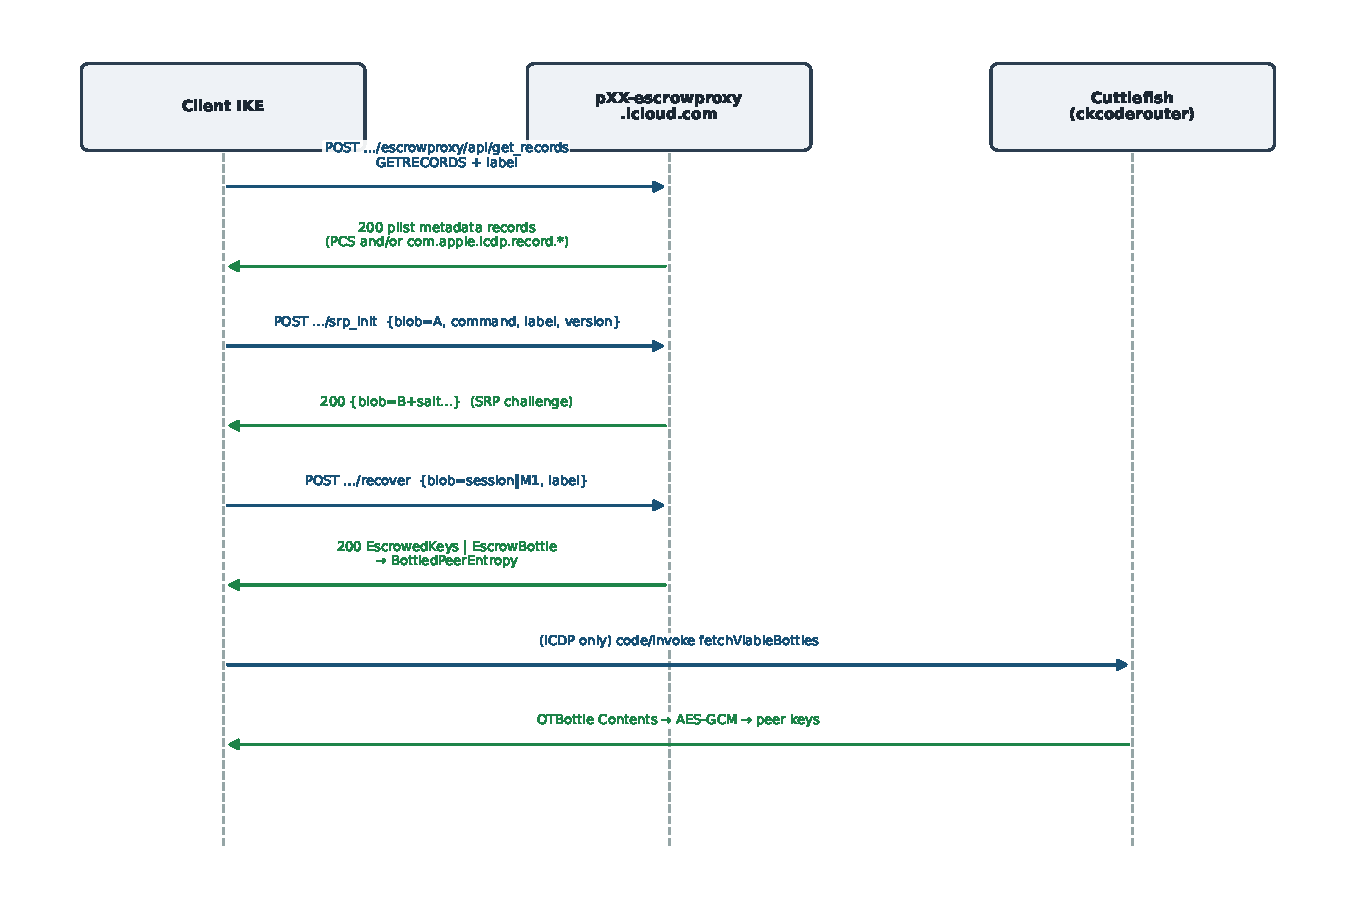
\includegraphics[keepaspectratio]{figures/fig07-seq-escrow.pdf}}

\textbf{Figure 7.} EscrowProxy sequence and, for iCDP, transition to
Cuttlefish \texttt{fetchViableBottles}.

\textbf{Endpoint:}
\texttt{POST\ https://\{partition\}-escrowproxy.icloud.com/escrowproxy/api/\{get\_records\textbar{}srp\_init\textbar{}recover\}}.

\textbf{Authentication:}

{\def\LTcaptype{none} % do not increment counter
\begin{longtable}[]{@{}
  >{\raggedright\arraybackslash}p{(\linewidth - 4\tabcolsep) * \real{0.2564}}
  >{\raggedright\arraybackslash}p{(\linewidth - 4\tabcolsep) * \real{0.3846}}
  >{\raggedright\arraybackslash}p{(\linewidth - 4\tabcolsep) * \real{0.3590}}@{}}
\toprule\noalign{}
\begin{minipage}[b]{\linewidth}\raggedright
Path
\end{minipage} & \begin{minipage}[b]{\linewidth}\raggedright
Authorization
\end{minipage} & \begin{minipage}[b]{\linewidth}\raggedright
Content-Type
\end{minipage} \\
\midrule\noalign{}
\endhead
\bottomrule\noalign{}
\endlastfoot
PCS Escrow & \texttt{X-MobileMe-AuthToken} + Basic(\texttt{dsid},
\texttt{mmeAuthToken}) & \texttt{text/x-xml-plist} \\
iCDP & \texttt{Basic} email + PET &
\texttt{application/x-apple-plist} \\
\end{longtable}
}

\textbf{Request --- get\_records:}

\begin{Shaded}
\begin{Highlighting}[]
\NormalTok{\textless{}}\KeywordTok{dict}\NormalTok{\textgreater{}}
\NormalTok{  \textless{}}\KeywordTok{key}\NormalTok{\textgreater{}command\textless{}/}\KeywordTok{key}\NormalTok{\textgreater{} \textless{}}\KeywordTok{string}\NormalTok{\textgreater{}GETRECORDS\textless{}/}\KeywordTok{string}\NormalTok{\textgreater{}}
\NormalTok{  \textless{}}\KeywordTok{key}\NormalTok{\textgreater{}label\textless{}/}\KeywordTok{key}\NormalTok{\textgreater{}   \textless{}}\KeywordTok{string}\NormalTok{\textgreater{}com.apple.protectedcloudstorage.record\textless{}/}\KeywordTok{string}\NormalTok{\textgreater{}}
  \CommentTok{\textless{}!{-}{-} oppure enumerazione label icdp: com.apple.icdp.record.* {-}{-}\textgreater{}}
\NormalTok{  \textless{}}\KeywordTok{key}\NormalTok{\textgreater{}version\textless{}/}\KeywordTok{key}\NormalTok{\textgreater{} \textless{}}\KeywordTok{integer}\NormalTok{\textgreater{}1\textless{}/}\KeywordTok{integer}\NormalTok{\textgreater{}}
\NormalTok{\textless{}/}\KeywordTok{dict}\NormalTok{\textgreater{}}
\end{Highlighting}
\end{Shaded}

\textbf{Response --- get\_records:} plist with metadata (serial, build,
remaining attempts, timestamp). No HSM consumption.

\textbf{Request --- srp\_init:}

\begin{Shaded}
\begin{Highlighting}[]
\NormalTok{\textless{}}\KeywordTok{dict}\NormalTok{\textgreater{}}
\NormalTok{  \textless{}}\KeywordTok{key}\NormalTok{\textgreater{}blob\textless{}/}\KeywordTok{key}\NormalTok{\textgreater{}    \textless{}}\KeywordTok{data}\NormalTok{\textgreater{}}\CommentTok{\textless{}!{-}{-} A SRP, 1..256 B {-}{-}\textgreater{}}\NormalTok{\textless{}/}\KeywordTok{data}\NormalTok{\textgreater{}}
\NormalTok{  \textless{}}\KeywordTok{key}\NormalTok{\textgreater{}command\textless{}/}\KeywordTok{key}\NormalTok{\textgreater{} \textless{}}\KeywordTok{string}\NormalTok{\textgreater{}SRP\_INIT\textless{}/}\KeywordTok{string}\NormalTok{\textgreater{}}
\NormalTok{  \textless{}}\KeywordTok{key}\NormalTok{\textgreater{}label\textless{}/}\KeywordTok{key}\NormalTok{\textgreater{}   \textless{}}\KeywordTok{string}\NormalTok{\textgreater{}com.apple.icdp.record.\textless{}}\KeywordTok{REDACTED}\NormalTok{\textgreater{}\textless{}/}\KeywordTok{string}\NormalTok{\textgreater{}}
\NormalTok{  \textless{}}\KeywordTok{key}\NormalTok{\textgreater{}version\textless{}/}\KeywordTok{key}\NormalTok{\textgreater{} \textless{}}\KeywordTok{integer}\NormalTok{\textgreater{}1\textless{}/}\KeywordTok{integer}\NormalTok{\textgreater{}}
\NormalTok{\textless{}/}\KeywordTok{dict}\NormalTok{\textgreater{}}
\end{Highlighting}
\end{Shaded}

\textbf{Request --- recover:} same fields with \texttt{command=RECOVER}
and \texttt{blob} = session material ‖ \texttt{M1}.

\textbf{Response --- recover (PCS):} material \textbf{EscrowedKeys} →
unwrap → \textbf{BackupBagPassword} → KeySet PCS.

\textbf{Response --- recover (iCDP):} \textbf{EscrowBottle} →
\textbf{BottledPeerEntropy} (\textasciitilde72 B). Next mandatory step:
Cuttlefish \texttt{fetchViableBottles} → Contents OTBottle → AES-GCM →
peer keys.

\begin{center}\rule{0.5\linewidth}{0.5pt}\end{center}

\subsubsection{13.3 Octagon / Cuttlefish /
CKKS}\label{octagon-cuttlefish-ckks}

\textbf{Sources:} \texttt{OctagonCuttlefishService.cs},
\texttt{OctagonRecoveryKeyUnlockService.cs},
\texttt{CkksVaultService.cs}.

\pandocbounded{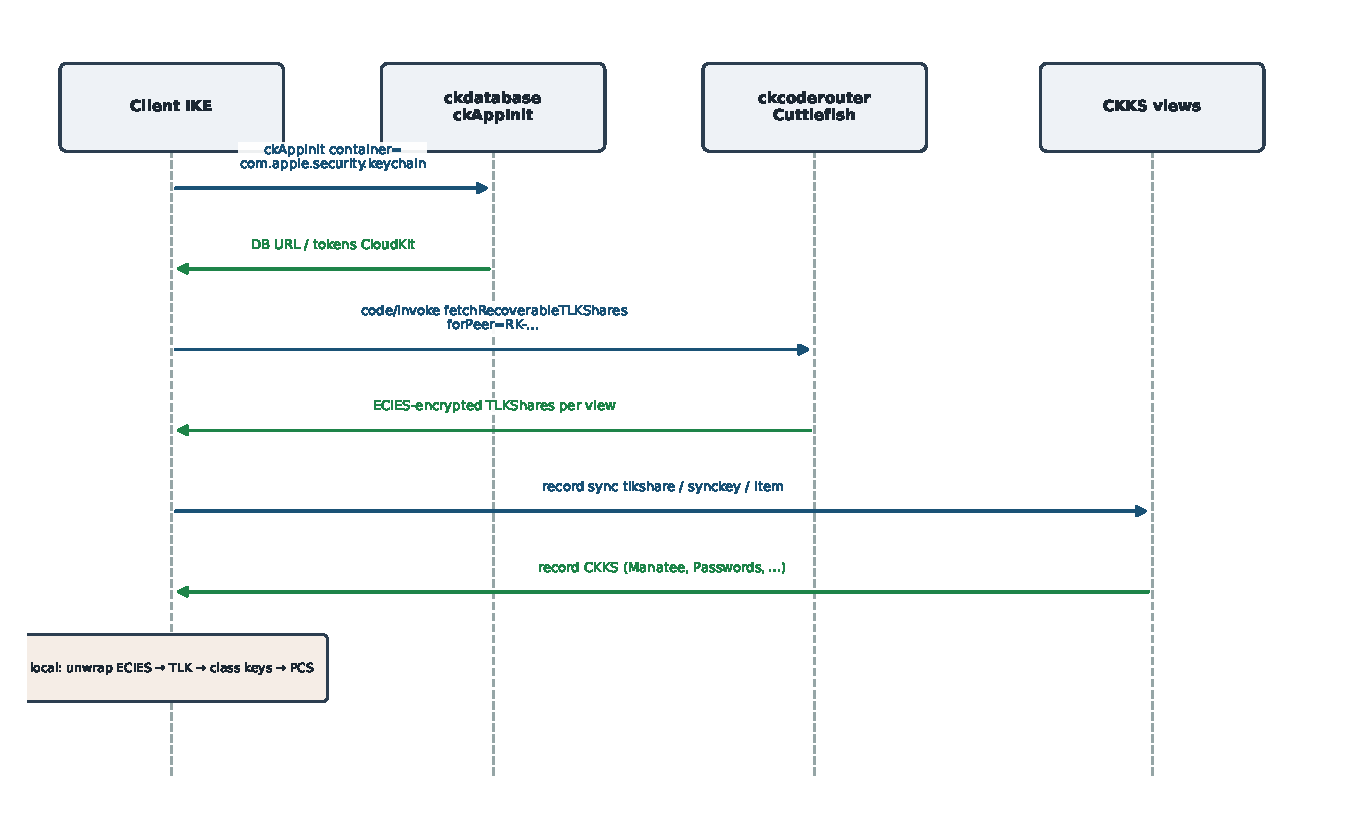
\includegraphics[keepaspectratio]{figures/fig08-seq-octagon-ckks.pdf}}

\textbf{Figure 8.} Recovery Key / peer →
\texttt{fetchRecoverableTLKShares} → opening view CKKS.

\textbf{Binding:}

\begin{itemize}
\tightlist
\item
  Container: \texttt{com.apple.security.keychain}
\item
  Bundle Cuttlefish: \texttt{com.apple.security.cuttlefish}
\item
  Gateway DB: \texttt{https://\{partition\}-ckdatabase.icloud.com}
\item
  Invoke: host \texttt{*-ckcoderouter.icloud.com}, operation
  \texttt{code/invoke}, service \texttt{Cuttlefish}
\end{itemize}

\textbf{Recovery Key steps (local + network):}

\begin{enumerate}
\def\labelenumi{\arabic{enumi}.}
\tightlist
\item
  Local:
  \texttt{HKDF-SHA384(IKM=UTF-8(RK),\ salt=UTF-8(altDSID),\ info=Recovery\ \{Signing\textbar{}Encryption\}\ Private\ Key)}
  → P-384 keys.
\item
  Peer ID = \texttt{RK-} + Base64(SHA-384(signing public key)).
\item
  Network: \texttt{ckAppInit} on the Keychain container.
\item
  Network: \texttt{fetchRecoverableTLKShares} with
  \texttt{forPeer=RK-…}.
\item
  Local: unwrap ECIES of TLKShare → TLK → class keys (\texttt{synckey})
  → item; extraction of PCS material from Manatee.
\end{enumerate}

\textbf{Semantic skeleton of the TLKShare response} (conceptual;
protobuf payload CloudKit):

\begin{verbatim}
functionInvokeResponse:
  recoverableTLKShares[]:
    view  = "Manatee" | "ProtectedCloudStorage" | "Passwords" | …
    wrappedKey = <ECIES blob toward peer RK-…>
\end{verbatim}

For the iCDP path, instead of the RK step, \texttt{fetchViableBottles}
appears after Escrow \texttt{RECOVER} (Figure 7).

\begin{center}\rule{0.5\linewidth}{0.5pt}\end{center}

\subsubsection{\texorpdfstring{13.4 CloudKit \texttt{mbksync} (catalog
and
Lock)}{13.4 CloudKit mbksync (catalog and Lock)}}\label{cloudkit-mbksync-catalog-and-lock}

\textbf{Sources:} \texttt{CloudKitGatewayClient.cs},
\texttt{CloudKitAssetService.cs}, \texttt{CloudKitLockRequestBuilder}.

\pandocbounded{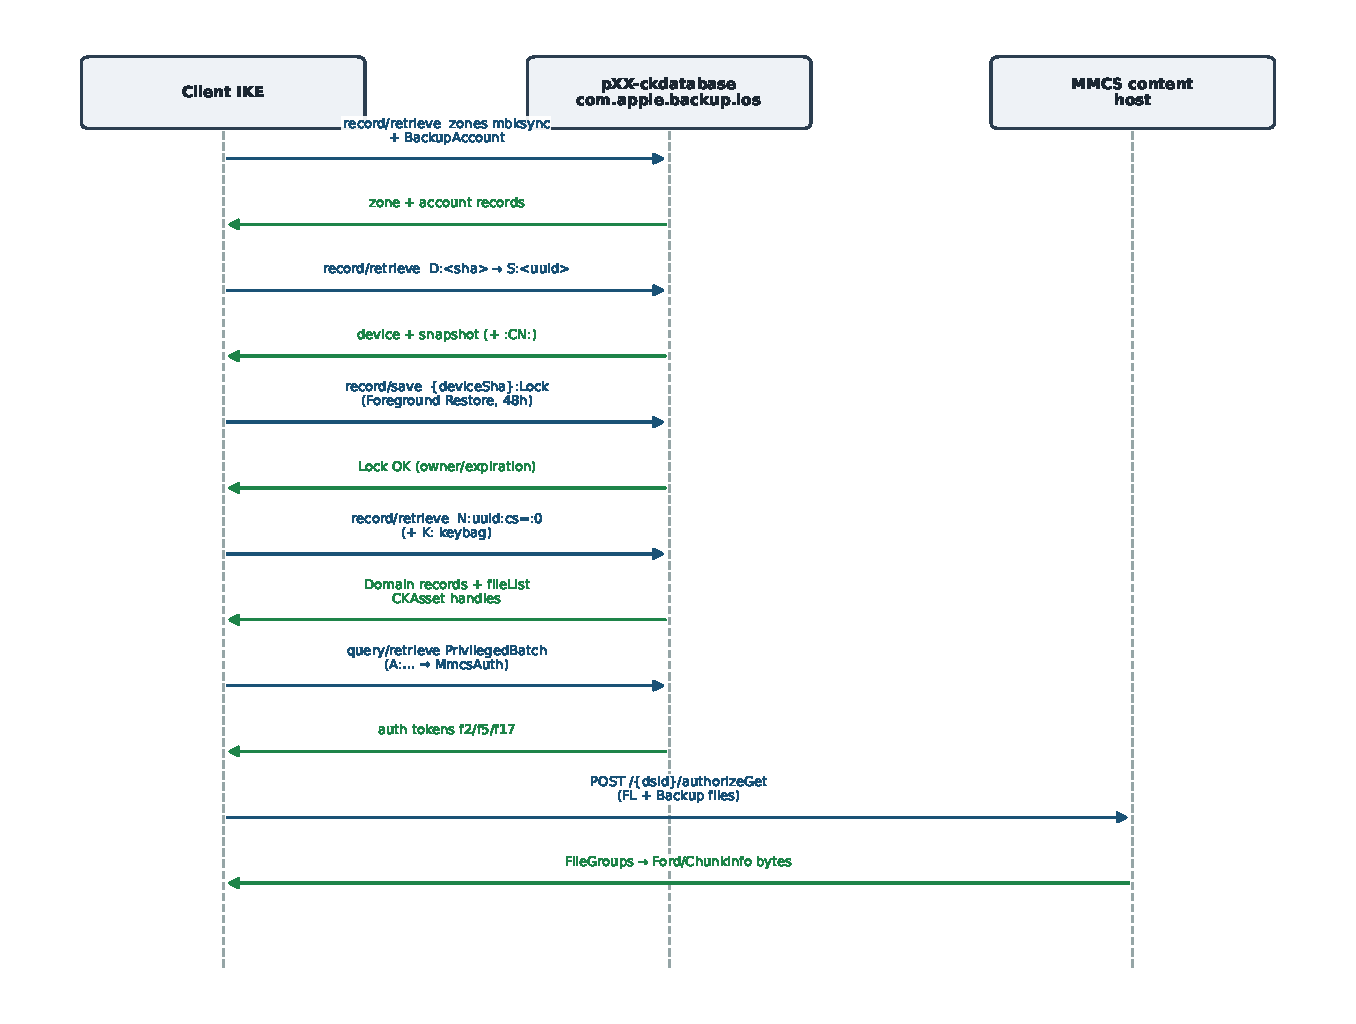
\includegraphics[keepaspectratio]{figures/fig09-seq-mbksync-mmcs.pdf}}

\textbf{Figure 9.} Backup inventory sequence: zones → D:/S: → Lock →
\texttt{N:} Domains → K: → PrivilegedBatch → MMCS (FL and files).

\textbf{Binding:}

\begin{itemize}
\tightlist
\item
  Container: \texttt{com.apple.backup.ios}
\item
  Bundle: \texttt{com.apple.backupd}
\item
  API:
  \texttt{POST\ https://\{partition\}-ckdatabase.icloud.com/api/client/\{record/retrieve\textbar{}record/save\textbar{}query/retrieve\textbar{}…\}}
\end{itemize}

\textbf{Invariant order} (client refuses to reorder):

\begin{verbatim}
zones → BackupAccount → D:<deviceSha> → S:<snapshotUuid>
  → (opt. MBS stub) → Lock → N:uuid:checksum=:0 → K:
\end{verbatim}

\textbf{Lock --- semantic skeleton} (\texttt{record/save}, type
\texttt{Lock}, zone \texttt{mbksync}):

\begin{verbatim}
recordName = "{deviceSha}:Lock"
owner      = "{deviceSha}"          # without D: prefix
duration   ≈ 172800 s (48 h)
metadata   ⊃ "Foreground Restore"  # later reflected in MMCS tokens (CAog…)
\end{verbatim}

\textbf{Negative Lock response typical:} string
\texttt{Invalid\ lock\ id} (often due to erroneous protobuf wrapping).

\textbf{Domain retrieve (post-Lock):} \texttt{record/retrieve} on
\texttt{N:…=:0} in \texttt{\_defaultZone} → Domain records with
\texttt{fileList} CKAsset handles (Section 9.5).

\textbf{PrivilegedBatch:} \texttt{query/retrieve} on record \texttt{A:…}
in \texttt{\_defaultZone} → extracts tokens that compose
\texttt{x-apple-mmcs-auth} (fields observed as f2/f5/f17) when flist
rows lack auth.

\begin{center}\rule{0.5\linewidth}{0.5pt}\end{center}

\subsubsection{\texorpdfstring{13.5 MMCS \texttt{authorizeGet} and edge
GET}{13.5 MMCS authorizeGet and edge GET}}\label{mmcs-authorizeget-and-edge-get}

\textbf{Sources:} \texttt{BackupDownloadService.cs}
(\texttt{AuthorizeGetAsync}), \texttt{Protocol/UbChunkBuilder.cs},
\texttt{FordMmcsDecryptor.cs}.

\pandocbounded{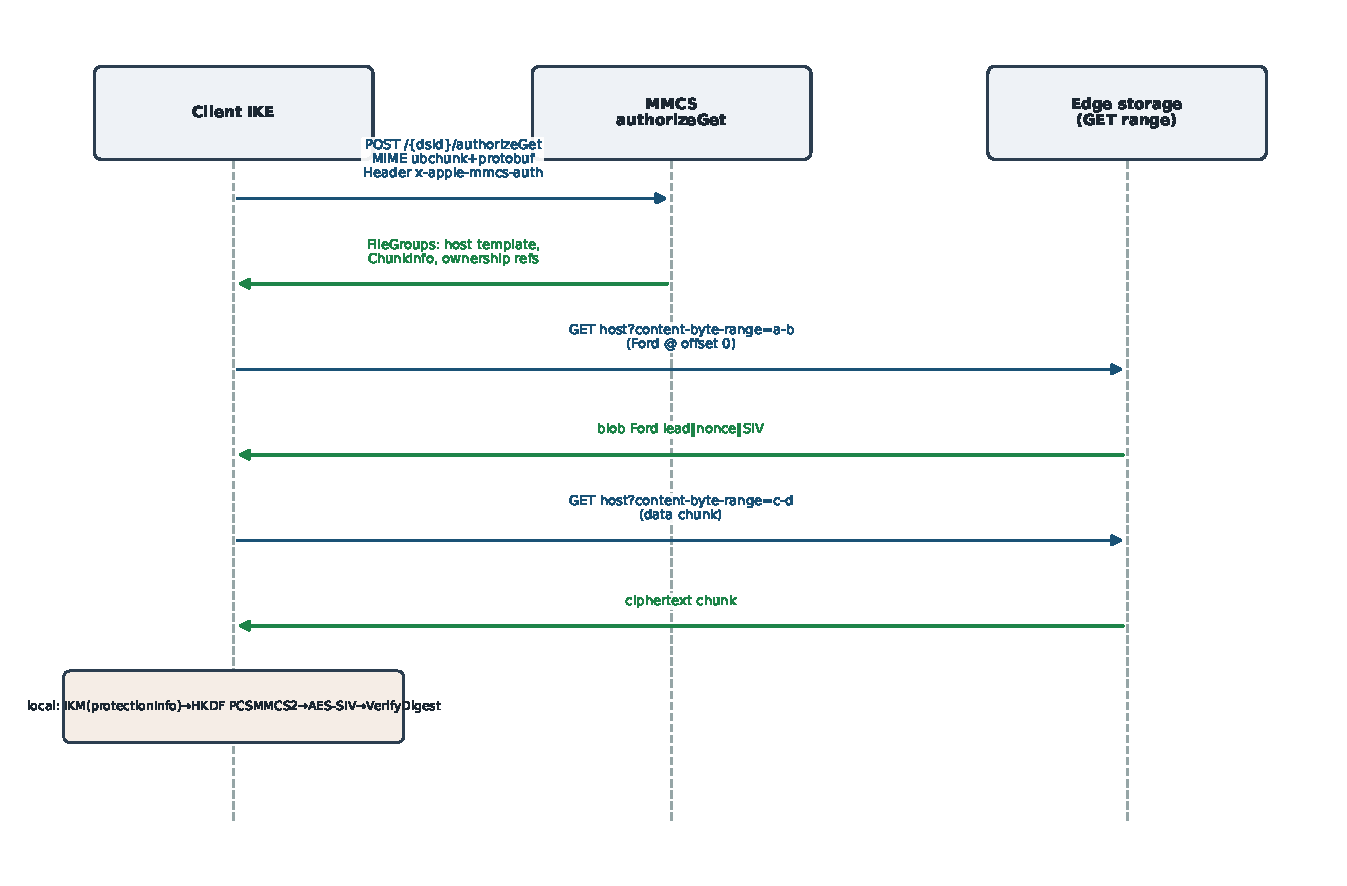
\includegraphics[keepaspectratio]{figures/fig10-seq-mmcs-detail.pdf}}

\textbf{Figure 10.} MMCS Detail: authorizeGet → FileGroups → ranged GET
→ local decryption.

\textbf{Request authorizeGet:}

\begin{verbatim}
POST https://{contentHost}/{dsid}/authorizeGet
Content-Type: application/vnd.com.apple.me.ubchunk+protobuf
Accept:       application/vnd.com.apple.me.ubchunk+protobuf
x-apple-mmcs-auth: <tok21hex> <tok21hex> <blobBase64url>
x-apple-mme-dsid: <dsid>
x-apple-mmcs-proto-version: 4.0
x-apple-mmcs-dataclass: com.apple.Dataclass.CloudKit
X-CloudKit-Container: com.apple.backup.ios
X-CloudKit-Zones: _defaultZone | mbksync
\end{verbatim}

Body: protobuf ubchunk constructed by
\texttt{UbChunkBuilder.BuildAuthorizeGetRequest} (typical batch ≤ 12
files).

\textbf{Response:} FileGroups with host template, ChunkInfo (checksum
21/45 B, \texttt{chunkEncryptionKey}, \texttt{ctLen}, offset) and
assembly references.

\textbf{Edge GET:}

\begin{verbatim}
GET https://{edgeHost}/…?content-byte-range={start}-{end}
\end{verbatim}

Same object: range including offset 0 → \textbf{Ford} material; other
ranges → data chunks.

\textbf{Local decryption (not network):}

\begin{verbatim}
IKM = unwrap(contents.protectionInfo, zoneMaster)
OKM = HKDF-SHA256(ikm=IKM, salt="PCSMMCS2", info="", len=64)
Ford = AES-SIV(OKM, AD=[nonce, lead])
chunk = ChunkDecrypt(…) + VerifyDigest
\end{verbatim}

\begin{center}\rule{0.5\linewidth}{0.5pt}\end{center}

\subsubsection{\texorpdfstring{13.6 File lists (Domain \texttt{N:} → FL
→ SQLite →
files)}{13.6 File lists (Domain N: → FL → SQLite → files)}}\label{file-lists-domain-n-fl-sqlite-files}

\textbf{Sources:} \texttt{BackupEnRecordService.cs},
\texttt{DomainFileListParser.cs}, \texttt{DomainPcsFieldDecryptor.cs},
\texttt{FileListSqliteParser.cs}, \texttt{FlistDownloadPlanBuilder.cs},
\texttt{BackupDownloadService.cs} (\texttt{ProcessOneDomainAsync} /
\texttt{MaterializeFileListDbAsync}).

\pandocbounded{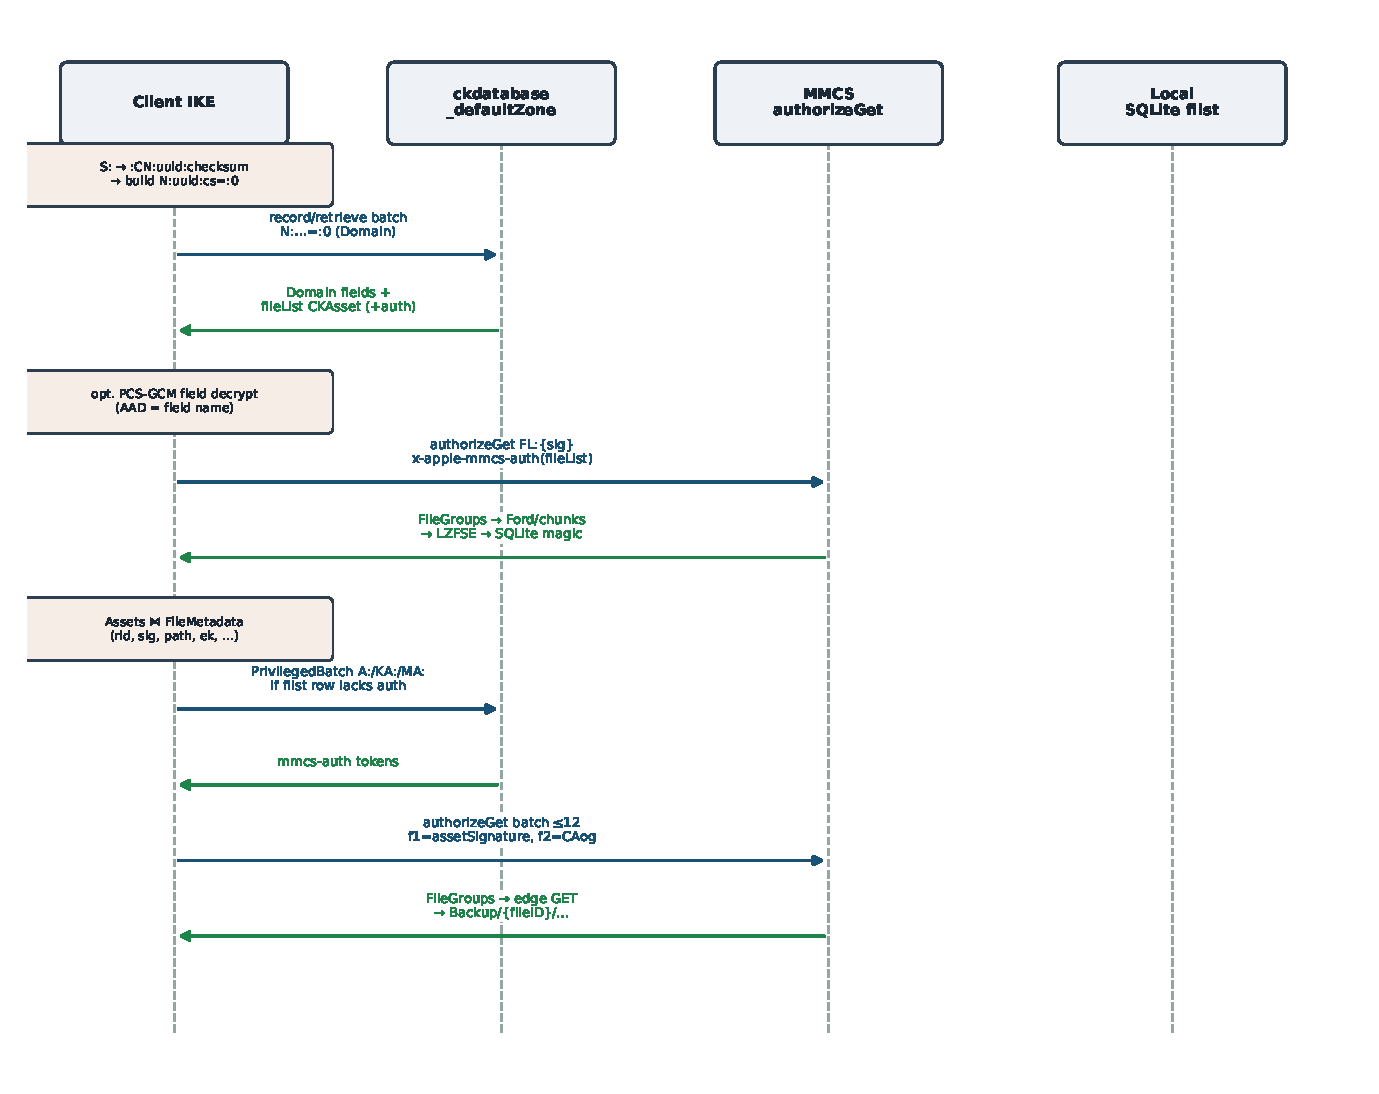
\includegraphics[keepaspectratio]{figures/fig11-seq-filelist.pdf}}

\textbf{Figure 11.} File-list path: \texttt{:CN:} → \texttt{N:} Domain
retrieve → MMCS download of \texttt{fileList} → LZFSE/SQLite → per-file
\texttt{authorizeGet} → Backup tree.

\textbf{Semantic skeleton --- Domain \texttt{fileList} CKAsset
(conceptual):}

\begin{verbatim}
recordName = "N:{uuid}:{checksum}=:0"     # _defaultZone; NOT "EN:…"
fields:
  domainName / domain
  fileListEncoding = 2                    # SQLite after expand
  fileList = CKAsset {
    signature21, size, contentBaseUrl,
    mmcsAuth = "{sigHex} {tok17Hex} {CAog…}",
    protectionWrap?
  }
\end{verbatim}

\textbf{Local expand (after Ford/\texttt{PCSMMCS2}):}

\begin{verbatim}
FL bytes → [LZFSE if bvx*] → "SQLite format 3"
  → Assets ⋈ FileMetadata
  → plan BackupAsset[] (skip dirs/symlinks/empty)
  → ensure mmcs-auth (PrivilegedBatch / PreAuth if needed)
  → authorizeGet batch (f1=assetSignature, f2=CAog, f4=companion)
  → edge GET → decrypt → Backup/{fileID[0..2]}/{fileID}
\end{verbatim}

\subsubsection{13.7 Global synthesis}\label{global-synthesis}

\begin{verbatim}
Anisette / MidService
  → GrandSlam init/complete (+ MFA)
  → setup.icloud.com (dsid, mmeAuthToken, partition)
  → Escrow GETRECORDS → SRP_INIT → RECOVER     [and/or RK → TLKShares]
  → (iCDP) fetchViableBottles → peer keys
  → open CKKS views / session PCS
  → mbksync zones → D: → S: → Lock → K:
  → N: Domains (from :CN:) → FL authorizeGet → SQLite flist
  → PrivilegedBatch (MmcsAuth) as needed
  → per-file authorizeGet → FileGroups → content-byte-range
  → Ford / ChunkDecrypt → iTunes-format tree
\end{verbatim}

Every arrow admits failure by design; the skeletons of this section are
intended for \textbf{forensic diagnosis} (which message, which field,
which stage).

\begin{center}\rule{0.5\linewidth}{0.5pt}\end{center}

\subsection{14. Conclusions}\label{conclusions}

The recovery of an iCloud backup under PCS/ADP is a
\textbf{concatenation of protocols}, not a single endpoint. GrandSlam
establishes the session; EscrowProxy and Cuttlefish provide semantically
distinct recovery paths; Octagon and CKKS (Manatee, TLKShare) supply the
material that makes \texttt{mbksync} and MMCS usable; Domain
\textbf{\texttt{N:}} / \textbf{fileList} records turn Lock into a path
inventory (SQLite flists); PCSMMCS2 and the Ford/ChunkInfo discipline
transform edge ranges into verified files.

The sequence diagrams and skeletons in Section 13 make the observable
messages on the protocol explicit by linking them to the IKE classes
that implement them.

For university instruction and forensic practice, the value lies in the
\textbf{explicit description of paths, invariants, and messages}, and in
the transparency of the method (Appendix A). The operational
result---iTunes tree on authorized accounts---is empirical evidence that
the map is sufficient, not proof that Apple will not modify it.

\begin{center}\rule{0.5\linewidth}{0.5pt}\end{center}

\subsection{15. Final Notes}\label{final-notes}

This white paper is deliberately focused on the \textbf{device-backup
acquisition chain} (GrandSlam → Escrow/Octagon/PCS → \texttt{mbksync} →
MMCS). It does not exhaust the scope of \emph{iCloudKit Extractor}.

In addition to this path, IKE uses and integrates --- as naming and flow
control, independently implemented in C\# and within the limits
specified in \texttt{NOTICE.md} {[}16{]} --- the same sources previously
cited in Section 16 to enhance the tool's completeness with respect to
other relevant iCloud surfaces in a forensic context:

{\def\LTcaptype{none} % do not increment counter
\begin{longtable}[]{@{}
  >{\raggedright\arraybackslash}p{(\linewidth - 4\tabcolsep) * \real{0.1714}}
  >{\raggedright\arraybackslash}p{(\linewidth - 4\tabcolsep) * \real{0.3429}}
  >{\raggedright\arraybackslash}p{(\linewidth - 4\tabcolsep) * \real{0.4857}}@{}}
\toprule\noalign{}
\begin{minipage}[b]{\linewidth}\raggedright
Surface
\end{minipage} & \begin{minipage}[b]{\linewidth}\raggedright
Role in IKE (summary)
\end{minipage} & \begin{minipage}[b]{\linewidth}\raggedright
Cited references
\end{minipage} \\
\midrule\noalign{}
\endhead
\bottomrule\noalign{}
\endlastfoot
\textbf{iCloud Keychain (CKKS)} & Opening CKKS views (Passwords, Wi‑Fi,
cert/keys, \ldots) after Octagon peer / TLKShare; see §15.1 & {[}7{]},
{[}8{]}, {[}9{]}, {[}11{]}, {[}12{]}, {[}14{]} \\
\textbf{Messages / iMessage in iCloud} & CloudKit / PCS / Engram-related
pathways to Messages & {[}6{]}, {[}13{]} \\
\textbf{Photos} & CloudKit sync and viewer-oriented materialization &
matrix {[}17{]}; lab notes {[}19{]} \\
\textbf{iCloud Drive} & Probe and pull documents & {[}2{]} (cloud drive
framing); {[}17{]}, {[}19{]} \\
\textbf{Voice Memos / Notes / Sync Data} & CloudKit sync zones beyond
\texttt{mbksync}; Voice Memos in the modern ADP-era flow --- see §15.2 &
{[}17{]}, {[}19{]}; PCS/Octagon from {[}11{]}--{[}14{]} \\
\textbf{WhatsApp / Mail / others} & Collateral paths documented in the
repository & {[}17{]}, {[}18{]} \\
\end{longtable}
}

\subsubsection{15.1 Keychain: Wi‑Fi network passwords (early November
2026)}\label{keychain-wifi-network-passwords-early-november-2026}

Along the CKKS path already outlined for Manatee / TLKShare, in
\textbf{early November 2026} the laboratory unlocked and decoded
\textbf{passwords of Wi‑Fi networks} stored in iCloud Keychain --- that
is, credentials of networks the device had joined and that were
synchronized into the relevant CKKS view (typically \texttt{WiFi} /
related SecItems). The result is not a separate protocol from
Octagon/CKKS: it is an operational consequence of opening the views with
a capable peer (iCDP passcode or Recovery Key) and interpreting the
resulting items. Passwords and related fields become available for
forensic review once the TLK / class-key unwrap succeeds; without that
material, the same records remain client-side ciphertext under ADP.

\subsubsection{15.2 Sync Data: Voice Memos in the modern (ADP)
flow}\label{sync-data-voice-memos-in-the-modern-adp-flow}

For \textbf{Sync Data} surfaces --- and \textbf{Voice Memos} in
particular --- practitioner feedback from digital forensic examiners who
compared currently available commercial products (including
\textbf{Magnet AXIOM Cyber}, \textbf{Elcomsoft Phone Breaker}, and
related offerings) indicates that \textbf{IKE is the first tool} they
observed able to acquire Voice Memos through the \textbf{contemporary
CloudKit / PCS sync path}, especially when \textbf{ADP is enabled}.
Commercial stacks often still rely on older sync assumptions,
web-oriented tokens, or restore-on-device workflows that omit or fail
this category under ADP. The claim here is framed as \textbf{field
comparison by practitioners}, not as a formal vendor-by-vendor audit
published in a venue paper; it is recorded because it clarifies IKE's
coverage relative to the backup-centric map of this document and
motivates keeping Sync Data (Voice Memos, Notes, \ldots) as a
first-class surface alongside \texttt{mbksync}.

In summary: this document's map makes the ADP-era remote backup
inspectable; disclosure {[}4{]}--{[}7{]}, Keychain documentation
{[}8{]}--{[}9{]}, and open-source projects {[}11{]}--{[}14{]} continue
to inform IKE beyond the iTunes tree --- including Keychain Wi‑Fi
credentials (§15.1) and modern Sync Data / Voice Memos (§15.2) ---
toward a more complete acquisition on authorized accounts, without
claiming product parity with every commercial tool on every category.

\begin{center}\rule{0.5\linewidth}{0.5pt}\end{center}

\subsection{16. References}\label{references}

\subsubsection{Literature review /
preprint}\label{literature-review-preprint}

{[}1{]} J. Geus, J. Ottmann, and F. Freiling, ``Systematic Evaluation of
Forensic Data Acquisition using Smartphone Local Backup,''
\emph{Proceedings of DFRWS USA}, 2023. Preprint:
\href{https://arxiv.org/abs/2404.12808}{arXiv:2404.12808}.

{[}2{]} V. Roussev, A. Barreto, and I. Ahmed, ``Forensic Acquisition of
Cloud Drives,'' in \emph{Advances in Digital Forensics XII}, G. Peterson
and S. Shenoi, Eds. Springer, 2016. Preprint:
\href{https://arxiv.org/abs/1603.06542}{arXiv:1603.06542}.

{[}3{]} M. Zinkus, T. M. Jois, and M. Green, ``Data Security on Mobile
Devices: Current State of the Art, Open Problems, and Proposed
Solutions,'' 2021. Preprint:
\href{https://arxiv.org/abs/2105.12613}{arXiv:2105.12613}.

\subsubsection{Industrial disclosures
(conferences)}\label{industrial-disclosures-conferences}

{[}4{]} V. Katalov, ``Cracking and Analyzing Apple's iCloud Protocol,''
\emph{Hack in the Box Security Conference (HITBSecConf)}, Kuala Lumpur,
2013. PDF:
\url{https://archive.conference.hitb.org/hitbsecconf2013kul/materials/D2T2\%20-\%20Vladimir\%20Katalov\%20-\%20Cracking\%20and\%20Analyzing\%20Apple's\%20iCloud\%20Protocol.pdf}.

{[}5{]} O. Afonin, ``Cracking and Analyzing Apple iCloud Backups, Find
My iPhone, Document Storage,'' \emph{REcon}, 2013. PDF:
\url{https://www.elcomsoft.fr/presentations/recon_2013.pdf}.

{[}6{]} V. Katalov, ``Cloudy With a Chance of Messages: Extracting
Messages from iCloud,'' \emph{HITBSecConf}, Dubai, 2018. PDF:
\url{https://conference.hitb.org/hitbsecconf2018dxb/materials/D1T2\%20-\%20Cloudy\%20With\%20a\%20Chance\%20of\%20Messages\%20-\%20Extracting\%20Messages\%20from\%20iCloud\%20-\%20Vladimir\%20Katalov.pdf}.

{[}7{]} V. Katalov, ``iCloud Keychain,'' \emph{SecTor}, 2017. PDF:
\url{https://archives.sector.ca/presentations17/vladimir-Katalov-iCloud_Keychain-(Katalov).pdf}

\subsubsection{Official documentation and
teaching}\label{official-documentation-and-teaching}

{[}8{]} Apple Inc., ``Escrow security for iCloud Keychain,'' \emph{Apple
Platform Security Guide}.
\url{https://support.apple.com/guide/security/escrow-security-for-icloud-keychain-sec3e341e75d/web}.

{[}9{]} Apple Inc., ``Secure iCloud Keychain recovery,'' \emph{Apple
Platform Security Guide}.
\url{https://support.apple.com/guide/security/secure-icloud-keychain-recovery-secdeb202947/web}.

{[}10{]} IAIK, Graz University of Technology, ``iOS Platform Security''
(course slides), 2024. PDF:
\url{https://www.isec.tugraz.at/wp-content/uploads/2023/09/2024-05-03-iOS-Platform-Security.pdf}.

\subsubsection{Software consulted and project
artifacts}\label{software-consulted-and-project-artifacts}

{[}11{]} Laky-64, \emph{appleservices} (MIT) --- cross-flow escrow iCDP
/ OTBottle / CKKS. \url{https://github.com/Laky-64/appleservices}

{[}12{]} Sank6, \emph{iCloud-Keychain-for-Linux} (MIT) --- notes on
KeyVault / Cuttlefish.
\url{https://github.com/Sank6/iCloud-Keychain-for-Linux}

{[}13{]} OpenBubbles, \emph{rustpush} (SSPL) --- PCS / Octagon study;
not redistributed in IKE. \url{https://github.com/OpenBubbles/rustpush}

{[}14{]} Apple open-source Security / TrustedPeersHelper --- KDF
Recovery Key / domain separation (Apple OSS)

{[}15{]} ElcomSoft, \emph{Elcomsoft Phone Breaker} --- experimental
observation on licensed builds; not OSS-dependent.

{[}16{]} G. Sconti, \emph{NOTICE.md} --- attribution and boundaries of
independent implementation.
\url{https://github.com/GiordanoSconti/iCloudKitExtractor/blob/main/NOTICE.md}

{[}17{]} G. Sconti, ``iCloud Acquisition Matrix (Windows),'' 8 November
2026.
\url{https://github.com/GiordanoSconti/iCloudKitExtractor/blob/main/docs/COMPARISON_ICLOUD_ACQUISITION.md}.

{[}18{]} G. Sconti, \emph{iCloudKit Extractor} (IKE) --- repository and
README. \url{https://github.com/GiordanoSconti/iCloudKitExtractor}

{[}19{]} G. Sconti, Laboratory experimental notes (Day 1--11) and
MMCS/protobuf maps, March--November 2026.
\url{https://giordanosconti.github.io/iCloudKitExtractor/}

{[}20{]} G. Sconti, ``Themida, x64dbg MCP, and Frida on memcpy,''
Experimental Lab note, 5 November 2026.
\url{https://giordanosconti.github.io/iCloudKitExtractor/blog/posts/2026-11-05-themida-x64dbg-mcp-frida-memcpy.html}.
Includes a link to the master's thesis used as a map:
\href{https://github.com/67-6f-64/AntiOreans-CodeDevirtualizer/blob/main/Masters\%20Thesis.pdf}{Masters
Thesis.pdf}
(\href{https://github.com/67-6f-64/AntiOreans-CodeDevirtualizer}{67-6f-64/AntiOreans-CodeDevirtualizer}).

{[}21{]} J. Geus, J. Gruber, J. Wozar, and F. Freiling, ``From sync to
seizure: A binary instrumentation-based evaluation of the iCloud backup
process,'' \emph{Forensic Science International: Digital Investigation},
vol.~54, 301978, 2025, doi:
\href{https://doi.org/10.1016/j.fsidi.2025.301978}{10.1016/j.fsidi.2025.301978}.
DFRWS APAC 2025. PDF:
\url{https://dfrws.org/wp-content/uploads/2025/10/From-sync-to-seizure-A-binary-instrumentatio_2025_Forensic-Science-Internat.pdf}.

{[}22{]} G. Sconti, ``Apple GrandSlam --- MidService provisioning (real
anisette),'' project documentation, 2026.
\url{https://github.com/GiordanoSconti/iCloudKitExtractor/blob/main/docs/APPLE_MIDSERVICE_PROVISIONING.md}.

{[}23{]} G. Sconti, ``Anisette and auth modes (reference iPhone vs
Docker),'' project documentation, 2026.
\url{https://github.com/GiordanoSconti/iCloudKitExtractor/blob/main/docs/MAC_ANISETTE.md}.

{[}24{]} G. Sconti, ``MMCS authorizeGet code map,'' Experimental Lab
note, 5 November 2026.
\url{https://giordanosconti.github.io/iCloudKitExtractor/blog/posts/2026-11-05-mmcs-authorizeget-code-map.html}.

{[}25{]} G. Sconti, ``Day 05 --- IKM from protectionInfo (not file-list
EncryptionKey),'' Experimental Lab note, 16 June 2026.
\url{https://giordanosconti.github.io/iCloudKitExtractor/blog/posts/2026-06-16-day-05-ikm.html}.

\begin{center}\rule{0.5\linewidth}{0.5pt}\end{center}

\section{Appendix A --- Reverse Engineering
Methodology}\label{appendix-a-reverse-engineering-methodology}

This appendix describes \textbf{how} the protocol chain was
reconstructed. It is an integral part of the whitepaper: without a
method, a description of the protocols would remain anecdotal. It does
not provide a redistributable software protection evasion procedure; it
outlines objectives, tools, chronological phases, and validation
criteria.

\subsection{A.1 Research question and ethical
constraints}\label{a.1-research-question-and-ethical-constraints}

\textbf{Question.} Which messages, orderings, and cryptographic
primitives are necessary and sufficient to acquire an iCloud backup
(with and without ADP) on authorized accounts, in a reproducible manner
in an independent client?

\textbf{Constraints.}

\begin{itemize}
\tightlist
\item
  Account / devices under control or mandate.
\item
  Legitimate license of the commercial client used as
  \textbf{observational reference}.
\item
  No redistribution of modified binaries.
\item
  Persistent output = labeled captures, invariant, and independent
  implementation (IKE).
\end{itemize}

\subsection{A.2 General Strategy}\label{a.2-general-strategy}

Three parallel pillars:

\begin{enumerate}
\def\labelenumi{\arabic{enumi}.}
\tightlist
\item
  \textbf{Commercial Observational Reference (EPB)} --- which network
  exchanges characterize a successful or failed restore (for example,
  403 with ADP)?
\item
  \textbf{Controlled device (jailbroken)} --- GrandSlam mobile,
  Anisette/\texttt{akd}, CloudKit names (\texttt{com.apple.backup.ios},
  \texttt{mbksync}) from the perspective of an authentic Apple client.
\item
  \textbf{Independent Client (IKE)} --- hypothesis → implementation →
  comparison with live captures → review when an invariant fails.
\end{enumerate}

Typical cycle: \emph{observe → formulate hypotheses on
field/organization → implement → repeat on laboratory account →
consolidate only what survives peer review}.

\subsection{A.3 Tools}\label{a.3-tools}

{\def\LTcaptype{none} % do not increment counter
\begin{longtable}[]{@{}
  >{\raggedright\arraybackslash}p{(\linewidth - 2\tabcolsep) * \real{0.6875}}
  >{\raggedright\arraybackslash}p{(\linewidth - 2\tabcolsep) * \real{0.3125}}@{}}
\toprule\noalign{}
\begin{minipage}[b]{\linewidth}\raggedright
Tool
\end{minipage} & \begin{minipage}[b]{\linewidth}\raggedright
Usage
\end{minipage} \\
\midrule\noalign{}
\endhead
\bottomrule\noalign{}
\endlastfoot
\textbf{x64dbg} (+ MCP bridge) & Prolonged sessions on protected Windows
clients; breakpoints on decode stubs; dumps of
post-virtualization/post-mutation regions \\
\textbf{Frida (Windows)} & Hook on \texttt{memcpy} (CRT VC++) to observe
HTTP/plist/protobuf buffers without relying exclusively on TLS pinning
violations \\
\textbf{Frida (iOS)} & Anisette Identity / \texttt{akd} on controlled
device \\
\textbf{Proxy / custom logging} & Once endpoints and MIME are known,
repeatable captures from the IKE client \\
\textbf{Note Day 1--11} & Experimental log: facts still valid on the
protocol vs.~hypotheses discarded \\
\end{longtable}
}

\subsubsection{A.3.1 Commercial client protection and reference
thesis}\label{a.3.1-commercial-client-protection-and-reference-thesis}

The commercial Windows client exhibited packing, API wrapping,
anti-debugging, virtualization, and instruction mutation. Prior to
devising a dedicated pathway, the preliminary study employed as a
\textbf{conceptual map} (not as an automatic unpacker) the master's
thesis on software obfuscation/protection and DBI-oriented recovery,
published in conjunction with the \emph{AntiOreans-CodeDevirtualizer}
project:

\begin{itemize}
\tightlist
\item
  PDF:
  \href{https://github.com/67-6f-64/AntiOreans-CodeDevirtualizer/blob/main/Masters\%20Thesis.pdf}{Masters
  Thesis.pdf}
\item
  Repository:
  \href{https://github.com/67-6f-64/AntiOreans-CodeDevirtualizer}{67-6f-64/AntiOreans-CodeDevirtualizer}
\end{itemize}

The attached tool code \textbf{was not} executed in the laboratory. From
the thesis, an operational vocabulary was derived:
\emph{write-then-execute} patterns, import reconstruction, PE dumping,
distinction between virtualization and mutation. The objective was not
to publish an unpacker, but to isolate the regions involving network and
cryptography. A dedicated laboratory note is provided in {[}20{]}.

\subsubsection{A.3.2 Recovery of native windows post-virtualization
(Themida-class)}\label{a.3.2-recovery-of-native-windows-post-virtualization-themida-class}

In virtualized environments, the interest logic is not readable as
static native code: it is executed by a protector's VM and, at certain
points, is \textbf{materialized} (even temporarily) as native bytes in
memory. The laboratory followed a repeatable cycle, guided by the thesis
checklist and x64dbg:

\begin{enumerate}
\def\labelenumi{\arabic{enumi}.}
\tightlist
\item
  \textbf{Classify the layer} --- packing / API wrapping / anti-debug /
  VM / mutation --- before investing time in the region.
\item
  \textbf{Identify the decode points} --- stubs that write to RWX
  regions or update VM handlers (pattern \emph{write-then-execute} from
  the thesis).
\item
  \textbf{Stop after transition} --- breakpoint on the decode stub /
  after the handler return; dump of the just-written memory window.
\item
  \textbf{Compare dumps across runs} --- retain only the buffers that
  occur in proximity to network calls or HTTP/plist buffers in
  subsequent sessions (correlation with Frida, §A.3.3).
\item
  \textbf{Annotate, do not redistribute} --- the dumps remain laboratory
  artifacts; in IKE only the protocol invariant (field, order, KDF)
  enters, not the reconstructed binary.
\end{enumerate}

\textbf{Operational example (abstract).} On a virtualized block that,
downstream, fed the construction of an EscrowProxy body:

\begin{itemize}
\tightlist
\item
  MCP on x64dbg set a breakpoint on the VM exit stub;
\item
  at the hit, dump of \(N\) KiB from the destination region of the
  write;
\item
  comparison with the dump from the previous run (same laboratory
  account, same Escrow flow);
\item
  if the dump contained recognizable strings (\texttt{command},
  \texttt{GETRECORDS}, \texttt{ProtectedCloudStorage}, plist prefixes)
  or fragments of SRP blobs, the region was marked as
  «protocol-relevant»; otherwise discarded as mutation noise.
\end{itemize}

In this sense, the observed ``decryption seed'' is not a publicly
releaseable Themida key, but rather the \textbf{runtime moment} at which
the protector has already generated (in memory) readable instructions or
buffers; by capturing that moment, one avoids fighting the entire VM as
a black box. The acceleration came from controlling x64dbg via
\textbf{MCP} with a coding assistant (reproducible dumps, triaging). The
judgment ``this block reveals an Apple RPC'' remained human.

\subsubsection{\texorpdfstring{A.3.3 Frida on \texttt{memcpy} (Windows):
message and secret PCS \texttt{dsid:dsid}
capture}{A.3.3 Frida on memcpy (Windows): message and secret PCS dsid:dsid capture}}\label{a.3.3-frida-on-memcpy-windows-message-and-secret-pcs-dsiddsid-capture}

Intercepting TLS end-to-end on a protected client proved intrusive
(pinning, stack customization, protector wrapper). Instrumenting
\textbf{\texttt{memcpy}} (and related CRT Visual C++ /
\texttt{ucrtbase}) revealed the body and headers at the moment they
existed as ordinary buffers---typically \emph{after} the application had
constructed the message and \emph{before} (or alongside) the TLS record.

\textbf{Filter schema used in the laboratory} (pseudocode; not a
redistributable attack script):

\begin{Shaded}
\begin{Highlighting}[]
\CommentTok{// Frida (Windows) — idea: hook memcpy del CRT, filtrare copie «interessanti»}
\NormalTok{Interceptor}\OperatorTok{.}\FunctionTok{attach}\NormalTok{(Module}\OperatorTok{.}\FunctionTok{findExportByName}\NormalTok{(}\StringTok{"ucrtbase.dll"}\OperatorTok{,} \StringTok{"memcpy"}\NormalTok{)}\OperatorTok{,}\NormalTok{ \{}
  \FunctionTok{onEnter}\NormalTok{(args) \{}
    \KeywordTok{const}\NormalTok{ n }\OperatorTok{=}\NormalTok{ args[}\DecValTok{2}\NormalTok{]}\OperatorTok{.}\FunctionTok{toInt32}\NormalTok{()}\OperatorTok{;}
    \ControlFlowTok{if}\NormalTok{ (n }\OperatorTok{\textless{}} \DecValTok{32} \OperatorTok{||}\NormalTok{ n }\OperatorTok{\textgreater{}} \DecValTok{2\_000\_000}\NormalTok{) }\ControlFlowTok{return}\OperatorTok{;}          \CommentTok{// scarta rumore}
    \KeywordTok{const}\NormalTok{ src }\OperatorTok{=}\NormalTok{ args[}\DecValTok{1}\NormalTok{]}\OperatorTok{;}
    \KeywordTok{const}\NormalTok{ head }\OperatorTok{=} \FunctionTok{hexdump}\NormalTok{(src}\OperatorTok{,}\NormalTok{ \{ }\DataTypeTok{length}\OperatorTok{:} \BuiltInTok{Math}\OperatorTok{.}\FunctionTok{min}\NormalTok{(n}\OperatorTok{,} \DecValTok{64}\NormalTok{)}\OperatorTok{,} \DataTypeTok{ansi}\OperatorTok{:} \KeywordTok{true}\NormalTok{ \})}\OperatorTok{;}
    \CommentTok{// Prefissi utili alle catture Apple:}
    \CommentTok{//  "POST ", "HTTP/1", "\textless{}?xml", "bplist", "command", "SRP\_INIT", …}
    \ControlFlowTok{if}\NormalTok{ (}\OperatorTok{!}\FunctionTok{looksLikeHttpOrPlistOrProtobuf}\NormalTok{(src}\OperatorTok{,}\NormalTok{ n)) }\ControlFlowTok{return}\OperatorTok{;}
    \FunctionTok{send}\NormalTok{(\{ }\DataTypeTok{len}\OperatorTok{:}\NormalTok{ n}\OperatorTok{,} \DataTypeTok{preview}\OperatorTok{:}\NormalTok{ head}\OperatorTok{,} \DataTypeTok{stack}\OperatorTok{:}\NormalTok{ Thread}\OperatorTok{.}\FunctionTok{backtrace}\NormalTok{(}\KeywordTok{this}\OperatorTok{.}\AttributeTok{context}\NormalTok{) \})}\OperatorTok{;}
    \CommentTok{// Opzionale: dump completo su file di laboratorio etichettato}
\NormalTok{  \}}
\NormalTok{\})}\OperatorTok{;}
\end{Highlighting}
\end{Shaded}

\textbf{Concrete example --- discovery/confirmation of
\texttt{dsid:dsid}.} During an Escrow PCS
(\texttt{label\ =\ ProtectedCloudStorage} / SecureBackup) flow,
intercepted buffers showed:

\begin{enumerate}
\def\labelenumi{\arabic{enumi}.}
\tightlist
\item
  Body plist of \texttt{SRP\_INIT} / \texttt{RECOVER} with fields
  \texttt{command}, \texttt{label}, \texttt{blob}, \texttt{version}.
\item
  During the same time interval, copies of UTF-8 strings of the form
  \texttt{\textless{}dsid\textgreater{}:\textless{}dsid\textgreater{}}
  (same numeric identifier on both sides of the \texttt{:}), used as the
  identity \texttt{I} and password \texttt{P} for the SRP computation
  --- \textbf{not} the device passcode.
\item
  Correlation with the response \texttt{srp\_init} (salt \texttt{s},
  public key \texttt{B}): repeated offline
\end{enumerate}

\begin{verbatim}
inner = SHA256( dsid ‖ ":" ‖ dsid )
x     = SHA256( salt ‖ inner )
\end{verbatim}

Produced an \texttt{M1} accepted by the server (ec≠−6015). The same
experiment with \texttt{dsid:passcode} failed on the PCS path and
succeeded on the iCDP path---empirical confirmation of the
\textbf{distinct-port taxonomy} (Section 6).

Other typical details emerged from the same hooks (always on laboratory
accounts):

{\def\LTcaptype{none} % do not increment counter
\begin{longtable}[]{@{}
  >{\raggedright\arraybackslash}p{(\linewidth - 2\tabcolsep) * \real{0.4894}}
  >{\raggedright\arraybackslash}p{(\linewidth - 2\tabcolsep) * \real{0.5106}}@{}}
\toprule\noalign{}
\begin{minipage}[b]{\linewidth}\raggedright
Observed in \texttt{memcpy}
\end{minipage} & \begin{minipage}[b]{\linewidth}\raggedright
Subsequent use in IKE
\end{minipage} \\
\midrule\noalign{}
\endhead
\bottomrule\noalign{}
\endlastfoot
Header Anisette \texttt{X-Apple-I-MD*} coherent init/complete &
\texttt{GrandSlamCpdBuilder} \\
PET / Basic \texttt{email:PET} toward escrowproxy & auth iCDP \\
\texttt{X-MobileMe-AuthToken} + dsid & auth PCS / CloudKit \\
MIME \texttt{application/vnd.com.apple.me.ubchunk+protobuf} &
\texttt{authorizeGet} \\
\texttt{CAog…} prefixes / 21-byte MMCS tokens &
\texttt{x-apple-mmcs-auth} \\
Record names \texttt{D:}, \texttt{S:}, \texttt{\{sha\}:Lock} &
\texttt{mbksync} order \\
\end{longtable}
}

\textbf{Frida on iOS} (distinct pillar): script under
\texttt{scripts/ios\_akd\_probe/} (\texttt{frida\_anisette.js},
\texttt{frida\_anisette\_lite.js}, IDS/HTTP captures) for minting
Anisette on \texttt{akd} and for validating CloudKit names from the
authentic Apple client --- not for bypassing Windows protection.

\subsection{A.4 Timeline of Discoveries (March--October
2026)}\label{a.4-timeline-of-discoveries-marchoctober-2026}

\subsubsection{A.4.1 March --- ADP, GrandSlam, initial backup
candidates}\label{a.4.1-march-adp-grandslam-initial-backup-candidates}

Requirement: backup with ADP. EPB did not fully address the case;
GrandSlam proved fragile even from the vendor side (subsequent fix).
Parallel paths: idmsa web (tokens inadequate for native clients) and
iPhone jailbroken (GrandSlam mobile + \texttt{mbksync}).

\textbf{Consolidated invariants:} init/complete GsService2 form; CPD
Anisette; binding \texttt{com.apple.backup.ios} / \texttt{mbksync}.

\subsubsection{A.4.2 April --- snapshot and
Lock}\label{a.4.2-april-snapshot-and-lock}

The \texttt{D:}/\texttt{S:} listing does not constitute a restore. The
lock on \texttt{mbksync} is a state requirement; Frida and
requested/response archived pairs enabled reconstruction of the machine
state. The lock was obtained \textbf{before} the
\texttt{backupProperties} decryption could proceed (which required
PCS/Octagon materials in October).

\textbf{Invariants:} order zones→Account→D:→S:→Lock→N:; Domain
\texttt{N:…=:0} (not literal \texttt{EN:}); Lock shape; duration; errors
\texttt{Invalid\ lock\ id}.

\subsubsection{A.4.3 May--July --- MMCS, IKM, Ford vs
ChunkInfo}\label{a.4.3-mayjuly-mmcs-ikm-ford-vs-chunkinfo}

After Lock: edge host, ranged GET, protobuf ubchunk. Critical result:
IKM from \textbf{\texttt{protectionInfo}}, not from the EncryptionKey in
the file list. During summer period: cache coherence issues (storing
every \texttt{0x04} corrupts \texttt{.chunks/}). Discipline: Ford only
with IKM; fixed fill order.

\textbf{Invariants:} MIME/header of authorizeGet; FileGroups; KDF
\texttt{PCSMMCS2}; AES-SIV Ford; ownership descriptors 45 B vs data
checksum 21 B.

\subsubsection{\texorpdfstring{A.4.4 August --- \texttt{0xC4} and the
iTunes
tree}{A.4.4 August --- 0xC4 and the iTunes tree}}\label{a.4.4-august-0xc4-and-the-itunes-tree}

Classification error: lead ≠ \texttt{0x04} does not imply ``Ford
invalid''. Data chunks with lead \texttt{0xC4} triggered download
protocol-complete. iTunes layout instantiation (\texttt{Manifest.db},
sidecars).

\subsubsection{A.4.5 October --- Octagon (passcode, then Recovery
Key)}\label{a.4.5-october-octagon-passcode-then-recovery-key}

MMCS could transfer ciphertext indefinitely; ADP decided whether to open
it. October 5: record iCDP + passcode. October 24: Recovery Key → peer
\texttt{RK-…} → TLKShares → Manatee. Unified material →
\texttt{backupProperties} and zones with ADP.

\subsection{A.5 Validation Criteria}\label{a.5-validation-criteria}

A fact enters the stable map only if:

\begin{enumerate}
\def\labelenumi{\arabic{enumi}.}
\tightlist
\item
  compare in independent captures / restore live;
\item
  survives IKE client revisions;
\item
  has a clear counterexample when violated (e.g., exchanged salt/info
  HKDF → Ford does not open; \texttt{M2} in complete → GSA error).
\end{enumerate}

Lab notes entry for Day 11 explicitly lists these facts. The present
white paper revisits the descriptive content in Sections 5--10.

\subsection{A.6 What the method does not
claim}\label{a.6-what-the-method-does-not-claim}

\begin{itemize}
\tightlist
\item
  Permanent stability of private APIs.
\item
  Completeness for every historical asset.
\item
  Equivalence between observation of EPB and possession of its source
  code.
\item
  Applicability of the same methodology to unauthorized accounts (it is
  neither ethically nor legally justified).
\end{itemize}

\subsection{A.7 Educational Transfer}\label{a.7-educational-transfer}

For a university course in security/forensics, the instructional
methodology is:

\begin{enumerate}
\def\labelenumi{\arabic{enumi}.}
\tightlist
\item
  separate the observational reference (observed behavior) from the
  independent implementation (own code);
\item
  use the literature on obfuscation/DBI (including the thesis in
  {[}20{]}) as a checklist, not as an unpack button;
\item
  correlate post-virtualization dumps and hook \texttt{memcpy} until a
  protocol invariant emerges (e.g., \texttt{dsid:dsid} vs
  \texttt{dsid:passcode});
\item
  version control hypotheses in an experimental log;
\item
  elevate to «protocol» only those invariants that survive
  counterproofs;
\item
  document paths and anti-patterns (Sections 6 and 12) regarding
  cryptographic primitives.
\end{enumerate}

\begin{center}\rule{0.5\linewidth}{0.5pt}\end{center}

\section{Appendix B --- Glossary}\label{appendix-b-glossary}

{\def\LTcaptype{none} % do not increment counter
\begin{longtable}[]{@{}
  >{\raggedright\arraybackslash}p{(\linewidth - 2\tabcolsep) * \real{0.4091}}
  >{\raggedright\arraybackslash}p{(\linewidth - 2\tabcolsep) * \real{0.5909}}@{}}
\toprule\noalign{}
\begin{minipage}[b]{\linewidth}\raggedright
Term
\end{minipage} & \begin{minipage}[b]{\linewidth}\raggedright
Definition
\end{minipage} \\
\midrule\noalign{}
\endhead
\bottomrule\noalign{}
\endlastfoot
GrandSlam / GSA & Apple ID Authentication via GsService2 + SRP-6a \\
CPD & \emph{Client provided data} (Anisette + device context) \\
PET & Post-login password equivalent token \\
dsid:dsid & SRP secret for the PCS Escrow path \\
EscrowProxy & Shared HSM Secure Backup transport for multiple recovery
paths \\
EscrowedKeys / KeySet & PCS material recovered from Escrow \\
BackupBagPassword & Post-SRP artifact to open the KeySet \\
iCDP bottle & Record Escrow \texttt{com.apple.icdp.record.*} \\
BottledPeerEntropy & \textasciitilde72 byte from EscrowBottle \\
OTBottle & Ciphertext Cuttlefish → peer keys \\
Octagon & ADP Trust Domain / Manatee / CKKS \\
Cuttlefish & Invoke service on \texttt{com.apple.security.keychain} \\
CKKS & CloudKit Keychain Syncing \\
TLK / TLKShare & CKKS view key and ECIES share key \\
Manatee & View CKKS → PCS material for ADP/backup \\
Engram & View CKKS associated to Messages; outside the backup path
described here \\
mbksync & CloudKit zone of the backup catalog \\
Lock & Session restore log on mbksync \\
authorizeGet & FileGroups MMCS Plan Authorization \\
PCSMMCS2 & Salt HKDF for Ford keys \\
Ford & AES-SIV key blobs on edge MMCS (term in {[}6{]}) \\
ChunkInfo & Data chunk descriptors (checksum, range, assembly) \\
ADP & Advanced Data Protection \\
Session PCS material & PCS keys available to the client for inventories
and MMCS \\
\end{longtable}
}

\end{document}
